\documentclass[12pt,a4paper]{report}

%==============================================================================
% PREAMBLE AND PACKAGES (Aligned with CEK / KTU B.Tech Project Format)
%==============================================================================
\usepackage{graphicx}
\usepackage{amsmath}
\usepackage{fancyhdr}
\usepackage{cite}
\usepackage{a4wide}
\usepackage{float}
\usepackage{epsfig}
\usepackage{longtable}
\usepackage{enumerate}
\usepackage{afterpage}
\usepackage{multirow}
\usepackage{ragged2e}
\usepackage{gensymb}
\usepackage{amsfonts} 
\usepackage[left=3.5cm,top=1.5cm,right=3cm,bottom=3cm]{geometry}
\usepackage{setspace}           
\usepackage{txfonts}
\usepackage{standalone}
\usepackage{tikz}
\usepackage{fontawesome5}
\usetikzlibrary{calc, shapes.geometric, arrows, arrows.meta, positioning, fit, backgrounds, shadows, tikzmark}

% Color definitions for TikZ diagrams (Clinical Deep Navy, Ocean Blue & Cyan Palette)
\definecolor{lavenderDark}{RGB}{15, 44, 89}
\definecolor{lavenderDeep}{RGB}{10, 28, 58}
\definecolor{lavenderMedium}{RGB}{29, 78, 158}
\definecolor{lavenderLight}{RGB}{240, 246, 255}
\definecolor{lavenderBorder}{RGB}{180, 205, 237}
\definecolor{lavenderAccent}{RGB}{2, 132, 199}
\definecolor{prismNavy}{RGB}{15, 44, 89}
\definecolor{prismBlue}{RGB}{29, 78, 158}
\definecolor{prismTeal}{RGB}{13, 148, 136}
\definecolor{prismMint}{RGB}{236, 253, 245}
\definecolor{prismGold}{RGB}{217, 119, 6}
\definecolor{prismDark}{RGB}{15, 23, 42}
\definecolor{prismLight}{RGB}{248, 250, 252}
\definecolor{prismIndigo}{RGB}{30, 58, 138}
\definecolor{prismSlate}{RGB}{100, 116, 139}
\definecolor{statusFail}{RGB}{220, 38, 38}
\definecolor{cInput}{RGB}{241, 245, 249}
\definecolor{cStem}{RGB}{224, 242, 254}
\definecolor{cStage1}{RGB}{209, 250, 229}
\definecolor{cStage2}{RGB}{254, 243, 199}
\definecolor{cStage3}{RGB}{254, 226, 226}
\definecolor{cStage4}{RGB}{207, 250, 254}
\definecolor{cHead}{RGB}{219, 234, 254}
\definecolor{cOutput}{RGB}{255, 228, 230}
\definecolor{cDeliverable}{RGB}{204, 251, 241}

\usepackage{subfiles}
\usepackage{adjustbox}
\usepackage{tcolorbox}
\tcbuselibrary{skins}

\newcommand{\Usefont}[1]{\fontfamily{#1}\selectfont}

\usepackage{lscape}
\linespread{1.5}

\usepackage{url}
\usepackage{subcaption}
\usepackage[intoc, english]{nomencl}
\usepackage[nottoc]{tocbibind}
\usepackage{booktabs}
\usepackage{array}
\usepackage{tabularx}
\usepackage{hyperref}

% Compact chapter-opening layout
\makeatletter
\def\@makechapterhead#1{%
  \vspace*{0pt}%
  {\parindent\z@ \raggedright \normalfont
    \ifnum\c@secnumdepth>\m@ne
      \huge\bfseries \@chapapp\space \thechapter
      \par\nobreak
      \vskip 10pt
    \fi
    \interlinepenalty\@M
    \Huge\bfseries #1\par\nobreak
    \vskip 15pt
  }}
\makeatother

\hypersetup{
    plainpages=false,
    pdfpagelabels=true,
    colorlinks=true,
    linkcolor=black,
    citecolor=black,
    urlcolor=black,
    pdftitle={AI-Powered Legal Information Retrieval using Retrieval-Augmented Generation},
    pdfauthor={Aleena AnilKumar, Abhinaya P S, Adithya Dinesh, Fathima A}
}

% Spacing and line-breaking settings to prevent overflow and overfull hboxes
\setlength{\headheight}{15pt}
\hyphenpenalty=1000
\tolerance=2000
\emergencystretch=2.5em

\bibliographystyle{IEEEtran}
\renewcommand{\bibname}{References}

% Figure search path
\graphicspath{{figures/}{diagrams/}{./}}

%==============================================================================
% METADATA DEFINITIONS (Project Group & CEK)
%==============================================================================
\gdef \title{AI-POWERED LEGAL INFORMATION RETRIEVAL USING RETRIEVAL-AUGMENTED GENERATION}
\gdef \shorttitle{AI-Powered Legal Information Retrieval using RAG}

\gdef \authorA{ALEENA ANILKUMAR}
\gdef \rollnoA{KNP23CS025}

\gdef \authorB{ABHINAYA P S}
\gdef \rollnoB{KNP23CO007}

\gdef \authorC{ADITHYA DINESH}
\gdef \rollnoC{KNP23CS016}

\gdef \authorD{FATHIMA A}
\gdef \rollnoD{KNP23CS047}

\gdef \acadyear{2026--2027}
\gdef \submonth{October 2026}
\gdef \month{October 2026}
\gdef \date{28-10-2026}
\gdef \dept{Computer Science and Engineering}
\gdef \deptabbr{Dept.\ of CSE}
\gdef \degree{Bachelor of Technology}
\gdef \branch{Computer Science and Engineering}
\gdef \college{College of Engineering Karunagappally}
\gdef \collegeplace{Kollam}
\gdef \collegetown{Karunagappally}

\gdef \guide{Ms. Hridhya J}
\gdef \guidedes{Assistant Professor}
\gdef \coordinator{Dr. Smitha P}
\gdef \coordinatordes{Associate Professor and HOD}
\gdef \semcordinatorA{Dr. Smitha P}
\gdef \semcordinatorAdes{Associate Professor and HOD}
\gdef \hod{Dr. Smitha P}
\gdef \hoddes{Associate Professor and HOD}

\providecommand{\candidateName}{\authorA}
\providecommand{\candidateRoll}{\rollnoA}

%==============================================================================
% DOCUMENT BODY
%==============================================================================

\begin{document}

%------------------------------------------------------------------------------
% FRONT MATTER
%------------------------------------------------------------------------------
\hypersetup{pageanchor=false}
%==================================coverpage.tex================================

\thispagestyle{empty}
\begin{titlepage}
\subfile{design_cover}
	\begin{center}\fontfamily{ptm}\selectfont
		{\Large \bfseries \title \par}
		\vspace*{12pt}
		{\large \Usefont{pzc}
			A PROJECT REPORT \par
			\vspace*{5pt}
			Submitted to the APJ Abdul Kalam Technological University \par
			\vspace*{5pt}
			in partial fulfillment of requirements for the award of degree\par}
		\vspace*{8pt}
		{\large \bfseries Bachelor of Technology}\par
		{\large in}\par
		{\large \bfseries \branch}\par
		\vspace*{10pt}
		{\large by}\par
		\vspace*{6pt}
		\begin{tabular}{l@{\hspace{1.8cm}}l}
			\large\bfseries ADHIL N         & \large\bfseries KNP23CS014 \\
			\large\bfseries ADARSH A S       & \large\bfseries KNP23CS010 \\
			\large\bfseries ADWAITH RAJ      & \large\bfseries KNP23CS019 \\
			\large\bfseries ABHISHEK SURESH  & \large\bfseries KNP23CS008
		\end{tabular}\par
		\vspace*{14pt}
		{
\includegraphics[width=4.0cm]{cek-logo.png}}\par
		\vspace{\stretch{0.5}}
		{\small \bfseries DEPARTMENT OF COMPUTER SCIENCE AND ENGINEERING}\par
		\vspace*{4pt}
		{\bfseries COLLEGE OF ENGINEERING KARUNAGAPPALLY}\par
		\vspace*{4pt}
		{\bfseries KOLLAM, KERALA}\par
		\vspace*{4pt}
		{\bfseries \submonth}\par
	\end{center}
\end{titlepage}

%=============================vision_mission.tex===============================
\thispagestyle{empty}

\begin{center}
    \vspace*{0.2cm}
    
\includegraphics[width=3.6cm]{cek-logo.png}\par
    \vspace*{0.5cm}
    {\bfseries\large COLLEGE OF ENGINEERING KARUNAGAPPALLY\par}
    \vspace*{0.2cm}
    {\bfseries Thodiyoor -- 690523\par}
    \vspace*{0.2cm}
    {\bfseries\large DEPARTMENT OF COMPUTER SCIENCE AND ENGINEERING\par}
    
    \vspace*{1.4cm}
    {\bfseries\large\underline{Vision of Department}\par}
    \vspace*{0.45cm}
    \begin{minipage}{0.92\linewidth}
        \centering
        To be renowned centre for education, research, and innovation in the frontier areas of Computer Science and Engineering.
    \end{minipage}\par

    \vspace*{1.4cm}
    {\bfseries\large\underline{Mission of Department}\par}
    \vspace*{0.5cm}
\end{center}

\noindent\hspace{0.02\linewidth}
\begin{minipage}{0.94\linewidth}
    \begin{itemize}
        \setlength\itemsep{1.1em}
        \item Establish and maintain an operational environment to acquire, impart, create and apply knowledge in Computer Science and Engineering and inter-disciplinary.
        \item Serve as a resource centre for innovation in design and development of hardware and software.
        \item Inculcate leadership qualities, professional ethics and a sense of social commitment.
    \end{itemize}
\end{minipage}

\vfill
\clearpage

%==================================certificate1.tex================================
% Certificate page for B.Tech Project Report

\newpage
\thispagestyle{empty}

\begin{spacing}{1.18}

\begin{center}
	\textbf{DEPARTMENT OF COMPUTER SCIENCE AND ENGINEERING}\\
	\textbf{COLLEGE OF ENGINEERING KARUNAGAPPALLY}\\
	\vspace*{3pt}
	\textbf{\acadyear}
\end{center}

\vspace*{6pt}
\begin{center}
	
\includegraphics[width=3.6cm]{cek-logo.png}
\end{center}

\vspace*{6pt}
\begin{center}
	\textbf{\Large CERTIFICATE}
\end{center}
\vspace*{8pt}

\noindent This is to certify that the report entitled \textbf{\title} submitted by \textbf{ADHIL N} (\rollnoA), \textbf{ADARSH A S} (\rollnoB), \textbf{ADWAITH RAJ} (\rollnoC), and \textbf{ABHISHEK SURESH} (\rollnoD), to the Department of \branch\ in partial fulfillment of the requirements for the award of the degree of Bachelor of Technology in \textbf{\branch}\ of the APJ Abdul Kalam Technological University is a bonafide record of the project work carried out by them under our guidance and supervision. This report in any form has not been submitted to any other University or Institute for any purpose.

\vspace*{2.0cm}

\noindent\begin{minipage}[t]{0.48\textwidth}
	\raggedright
	\textbf{Mrs. Swathi S} \\
	(Project Guide) \\
	Assistant Professor \\
	Dept. of CSE \\
	CE, Karunagappally
\end{minipage}\hfill
\begin{minipage}[t]{0.48\textwidth}
	\raggedright
	\textbf{Dr. Smitha P} \\
	(Project Coordinator) \\
	Associate Professor and HOD \\
	Dept. of CSE \\
	CE, Karunagappally
\end{minipage}

\end{spacing}

\thispagestyle{empty}
%============================================================================

%==================================certificate_individual.tex================================
% Individual Certificate page for B.Tech Project Report
\newpage
\thispagestyle{empty}

\begin{spacing}{1.18}

\begin{center}
	\textbf{DEPARTMENT OF COMPUTER SCIENCE AND ENGINEERING}\\
	\textbf{COLLEGE OF ENGINEERING KARUNAGAPPALLY}\\
	\vspace*{3pt}
	\textbf{\acadyear}
\end{center}

\vspace*{6pt}
\begin{center}
	
\includegraphics[width=3.6cm]{cek-logo.png}
\end{center}

\vspace*{6pt}
\begin{center}
	\textbf{\Large CERTIFICATE}
\end{center}
\vspace*{8pt}

{\sloppy
\hyphenpenalty=10000
\exhyphenpenalty=10000
\noindent This is to certify that the report entitled \textbf{\title} submitted by \textbf{\candidateName} (\candidateRoll), to the Department of \branch\ in partial fulfillment of the requirements for the award of the degree of Bachelor of Technology in \textbf{\branch}\ of the APJ Abdul Kalam Technological University is a bonafide record of the project work carried out by him under our guidance and supervision. This report in any form has not been submitted to any other University or Institute for any purpose.\par}

\vspace*{2.0cm}

\noindent\begin{minipage}[t]{0.48\textwidth}
	\raggedright
	\textbf{Mrs. Swathi S} \\
	(Project Guide) \\
	Assistant Professor \\
	Dept. of CSE \\
	CE, Karunagappally
\end{minipage}\hfill
\begin{minipage}[t]{0.48\textwidth}
	\raggedright
	\textbf{Dr. Smitha P} \\
	(Project Coordinator) \\
	Associate Professor and HOD \\
	Dept. of CSE \\
	CE, Karunagappally
\end{minipage}

\end{spacing}

\thispagestyle{empty}
%============================================================================

%==================================declaration.tex================================
\newpage
\thispagestyle{empty}

\begin{center}
\vspace*{24pt}
\textbf{\Large DECLARATION}\\[18pt]
\end{center}

{\fontsize{12.5pt}{18pt}\selectfont
\begin{spacing}{1.15}
\noindent We, \textbf{ADHIL N} (\rollnoA), \textbf{ADARSH A S} (\rollnoB), \textbf{ADWAITH RAJ} (\rollnoC), and \textbf{ABHISHEK SURESH} (\rollnoD), hereby declare that the project report entitled \textbf{\title}, submitted for partial fulfillment of the requirements for the award of the degree of Bachelor of Technology in \branch\ of the APJ Abdul Kalam Technological University, Kerala, is a bonafide work done by us under the supervision of \mbox{\textbf{\guide}} (\guidedes, \deptabbr, \college).\par
\vspace{10pt}
\noindent This submission represents our ideas in our own words, and where ideas or words of others have been included, we have adequately and accurately cited and referenced the original sources.\par 
\vspace{10pt}
\noindent We also declare that we have adhered to the ethics of academic honesty and integrity and have not misrepresented or fabricated any data, idea, fact, or source in our submission. We understand that any violation of the above will be a cause for disciplinary action by the Institute and/or the University and can also evoke penal action from the sources which have thus not been properly cited or from whom proper permission has not been obtained. This report has not previously formed the basis for the award of any degree, diploma, or similar title of any other University or Institute.
\end{spacing}}

\vspace{1.55cm}

\noindent \begin{minipage}{0.40\linewidth}
\fontsize{12.5pt}{18pt}\selectfont
\begin{flushleft}
\textbf{\collegetown} \\
\textbf{\date}
\end{flushleft} 
\end{minipage}
\hfill
\begin{minipage}{0.56\linewidth}
\fontsize{12.5pt}{18pt}\selectfont
\begin{flushright}                                      
\textbf{ADHIL N} (\rollnoA) \\[4pt]
\textbf{ADARSH A S} (\rollnoB) \\[4pt]
\textbf{ADWAITH RAJ} (\rollnoC) \\[4pt]
\textbf{ABHISHEK SURESH} (\rollnoD)
\end{flushright} 
\end{minipage}

\thispagestyle{empty}

\hypersetup{pageanchor=true}

\cleardoublepage
\pagenumbering{roman}
\pagestyle{plain}

%============================= abstract.tex================================
\chapter*{Abstract}%
\addcontentsline{toc}{chapter}{Abstract}%
\vspace{-25pt}

\begin{spacing}{1.2}
\noindent Security and surveillance networks face critical operational bottlenecks due to the computational demands and lack of end-to-end integration between anomaly detection and multi-camera tracking systems. Traditional deep learning architectures, particularly 3D Convolutional Neural Networks (3D CNNs), are prohibitively power-intensive for continuous 24/7 surveillance at the edge, while existing person tracking and re-identification systems typically operate as disconnected, continuous pipelines that process redundant video feeds indiscriminately. 

\vspace{8pt}

\noindent To address these challenges, this project presents an end-to-end neuromorphic edge intelligence framework that couples a hybrid \textbf{CNN--Spiking Neural Network (SNN)} anomaly detection module with an \textbf{event-triggered multi-camera person tracking} subsystem. The anomaly detection module (System~A) continuously monitors surveillance streams using a lightweight \textbf{MobileNetV3-Large} spatial backbone coupled with spatial attention, projecting frame embeddings into a dual-timescale spiking temporal processor composed of \textbf{Parametric Leaky Integrate-and-Fire (PLIF)} neurons trained with surrogate gradient backpropagation. When an anomalous event is detected with confidence exceeding a calibrated threshold ($\theta_a = 0.521$), System~A writes cropped suspect images and spatial-temporal metadata to a structured query registry, dynamically activating the multi-camera tracking subsystem (System~B). System~B executes two-tier \textbf{YOLOv8n} person detection, two-stage \textbf{ByteTrack} association with Kalman filtering, crop quality validation with CLAHE enhancement, and omni-scale re-identification feature extraction via \textbf{OSNet-AIN}. Robust identity matching across disjoint camera views is achieved through \textbf{Mahalanobis-filtered tracklet feature centralization} and cosine distance comparison.

\vspace{8pt}

\noindent Comprehensive empirical evaluations on the \textbf{UCF-Crime} dataset demonstrate that the proposed anomaly detection module achieves an accuracy of \textbf{90.11\%}, recall of \textbf{91.61\%}, and an \textbf{AUC-ROC of 0.9557}, while consuming only \textbf{3.1\,W} (13.34\,W peak on an NVIDIA T4 GPU), representing an \textbf{87\% energy reduction} over standard 3D CNN baselines. The event-triggered gating policy reduces downstream tracking computations by \textbf{94\%} and network bandwidth by \textbf{96.5\%}, maintaining real-time edge execution at \textbf{28\,FPS}. On the DukeMTMC re-identification benchmark structured for tracklet continuity, the proposed tracklet centralization pipeline achieves a \textbf{Rank-1 accuracy of 94.02\%} and \textbf{mAP of 86.62\%}, establishing a privacy-preserving, highly scalable, and energy-efficient solution for intelligent surveillance.
\end{spacing}

\thispagestyle{plain}
%=======================================================================

%==================================acknowledgement.tex=============================
\chapter*{Acknowledgement}%
\addcontentsline{toc}{chapter}{Acknowledgement}%
\vspace{-15pt}

\begin{spacing}{1.25}
\noindent We take this opportunity to express our deepest gratitude and sincere thanks to everyone who helped us to complete this project work and report successfully.

\vspace{6pt}

\noindent We express our sincere thanks to \mbox{\textbf{Dr.~Smitha P}}, Principal in-charge / Head of Department, \dept, \college, \collegeplace, for providing us with all the necessary infrastructural facilities, high-performance computing resources, and institutional encouragement.

\vspace{6pt}

\noindent We would like to express our profound sense of gratitude and indebtedness to our project guide \mbox{\textbf{\guide}}, \guidedes, \dept, \college, for her insightful guidance, constant encouragement, rigorous critiques, and invaluable mentorship throughout the entire lifecycle of this project.

\vspace{6pt}

\noindent We also express our sincere gratitude and indebtedness to our project coordinator \mbox{\textbf{\coordinator}}, \coordinatordes, \dept, \college, for her continuous coordination, constructive reviews, and valuable support during each phase of this project.

\vspace{6pt}

\noindent We also convey our sincere appreciation to all the faculty members and technical staff of the \dept\ for their kind cooperation, constructive academic advice, and technical support during our design and development phases.

\vspace{6pt}

\noindent Finally, we express our wholehearted thanks to our parents, family members, and friends who provided unwavering moral support, patience, and encouragement that contributed immensely to the successful realization of this project.

\vspace*{14pt}
\begin{flushright}
	\textbf{ADHIL N} (\rollnoA) \\[3pt]
	\textbf{ADARSH A S} (\rollnoB) \\[3pt]
	\textbf{ADWAITH RAJ} (\rollnoC) \\[3pt]
	\textbf{ABHISHEK SURESH} (\rollnoD)
\end{flushright}
\end{spacing}

\thispagestyle{plain}


\cleardoublepage
\tableofcontents
\cleardoublepage
\listoffigures
\cleardoublepage
\listoftables
\cleardoublepage

%==================================symbol.tex================================
% List of Symbols and Abbreviations
\chapter*{List of Symbols and Abbreviations}
\addcontentsline{toc}{chapter}{List of Symbols and Abbreviations}%
\vspace{-25pt}

\begin{spacing}{1.02}
\noindent \textbf{Abbreviations}
\vspace{4pt}

\noindent\begin{tabular*}{\textwidth}{@{\extracolsep{\fill}}p{2.8cm} p{11.2cm}@{}}
\textbf{SNN} & Spiking Neural Network \\
\textbf{CNN} & Convolutional Neural Network \\
\textbf{ANN} & Artificial Neural Network \\
\textbf{PLIF} & Parametric Leaky Integrate-and-Fire \\
\textbf{LIF} & Leaky Integrate-and-Fire \\
\textbf{BPTT} & Backpropagation Through Time \\
\textbf{YOLO} & You Only Look Once \\
\textbf{MOT} & Multi-Object Tracking \\
\textbf{Re-ID} & Person Re-Identification \\
\textbf{MTMCT} & Multi-Target Multi-Camera Tracking \\
\textbf{IoU} & Intersection over Union \\
\textbf{CLAHE} & Contrast Limited Adaptive Histogram Equalization \\
\textbf{OSNet} & Omni-Scale Network \\
\textbf{AIN} & Attentive Instance Normalization \\
\textbf{AUC-ROC} & Area Under Receiver Operating Characteristic Curve \\
\textbf{FPS} & Frames Per Second \\
\textbf{GPU} & Graphics Processing Unit \\
\textbf{GMM} & Gaussian Mixture Model \\
\textbf{GFLOPs} & Giga Floating-Point Operations per Second \\
\textbf{DFD} & Data Flow Diagram \\
\textbf{SRS} & System Requirements Specification \\
\textbf{mAP} & Mean Average Precision \\
\end{tabular*}

\vspace{6pt}
\noindent \textbf{Mathematical Notations}
\nopagebreak[4]
\vspace{4pt}
\nopagebreak[4]

\noindent\begin{tabular*}{\textwidth}{@{\extracolsep{\fill}}p{2.8cm} p{11.2cm}@{}}
$V[t]$ & Membrane potential of the spiking neuron at discrete time step $t$ \\
$\tau$ & Membrane potential decay time constant in PLIF neuron dynamics \\
$V_{\text{th}}$ & Fixed firing threshold potential for action potential emission \\
$\Theta(\cdot)$ & Heaviside unit step function generating discrete spike activity \\
$S[t]$ & Binary spike emission state at time $t$ ($S[t] \in \{0, 1\}$) \\
$\sigma'(x)$ & Continuous surrogate gradient derivative used during backpropagation \\
$z_t$ & Projected 256-dimensional spatial feature vector at frame step $t$ \\
$S_f(t), S_s(t)$ & Discrete spike trains generated from fast and slow temporal pathways \\
$g_t$ & Learnable adaptive gating coefficient fusing dual-timescale pathways \\
$h_t$ & Fused temporal spiking feature representation at time step $t$ \\
$\alpha_t$ & Normalized temporal attention weight allocated to frame step $t$ \\
$h_{\text{video}}$ & Final unified temporal feature representation for video clip \\
$\theta_a$ & Operational decision threshold for anomaly triggering ($\theta_a = 0.521$) \\
$\theta_s$ & Cosine similarity threshold for cross-camera Re-ID match ($\theta_s = 0.75$) \\
$\mathbf{c}_q$ & Centralized 512-dimensional query person identity vector \\
$\mathbf{c}_g$ & Centralized 512-dimensional gallery tracklet identity vector \\
$\text{sim}(\mathbf{c}_q, \mathbf{c}_g)$ & Cosine similarity score between query and gallery identity embeddings \\
$N^*$ & Number of valid candidate frames retained after Mahalanobis outlier filtering \\
$D_i$ & Person detection candidate tuple $(x_1, y_1, x_2, y_2, c_i)$ with bounding box and score \\
$\mathcal{L}_{\text{video}}$ & Class-weighted focal loss evaluated on video-level anomaly classification \\
$\mathcal{L}_{\text{frame}}$ & Frame-level focal loss supervising temporal anomaly predictions \\
\end{tabular*}
\end{spacing}

\thispagestyle{plain}
%=======================================================================


%------------------------------------------------------------------------------
% MAIN BODY (Arabic Numbering & Header/Footer)
%------------------------------------------------------------------------------
\cleardoublepage
\setcounter{page}{1}
\pagenumbering{arabic}

\pagestyle{fancy}
\fancyhf{}
\fancyhead[L]{\fontsize{9}{11}\selectfont \textit{\shorttitle}}
\fancyhead[R]{\fontsize{9}{11}\selectfont \textit{\deptabbr, CEK}}
\fancyfoot[C]{\thepage}
\renewcommand{\headrulewidth}{0.4pt}
\renewcommand{\footrulewidth}{0pt}

%==============================================================================
% CHAPTER 1: INTRODUCTION
%==============================================================================
\chapter[Introduction]{\Huge Introduction}

Access to accurate, comprehensible legal information is fundamental to civic empowerment and the effective exercise of constitutional rights in India. Citizens encounter legal systems daily—from consumer disputes and service grievances to information access rights under the Right to Information (RTI) Act 2005 and criminal proceedings under the Bharatiya Nyaya Sanhita (BNS) 2023. However, contemporary legal information retrieval faces systemic obstacles:

\begin{enumerate}[(i)]
    \item \textbf{Statutory Language Complexity:} Legal texts employ specialized terminology, nested conditional clauses, and cross-references that are impenetrable to non-lawyers.
    \item \textbf{Fragmented Document Repositories:} Statutes, amendments, judicial interpretations, and procedural codes are scattered across government portals, parliamentary archives, and district registries without unified search.
    \item \textbf{Language Barriers:} Over 57\% of Indian citizens speak regional languages as their primary tongue, yet most legal resources remain exclusively in English or technical Hindi, excluding Malayalam, Tamil, Telugu, and other linguistic communities.
    \item \textbf{Lack of Contextual Answers:} Traditional keyword search returns raw statutory clauses without explanation of applicability, penalties, or procedural steps, requiring expensive legal consultation.
\end{enumerate}

To address these challenges, this project presents \textbf{CiviQ – AI-Powered Civic Issue Reporting and Complaint Management System}, a Retrieval-Augmented Generation (RAG) platform for citizen-accessible legal information retrieval. The system ingests comprehensive legal corpora including BNS 2023, BNSS 2023, BSA 2023, Consumer Protection Act 2019, Indian Contract Act 1872, RTI Act 2005, and the Constitution of India. Documents are preprocessed through overlapping word-chunking (900-word chunks, 150-word overlap), embedded via \textbf{sentence-transformers (all-MiniLM-L6-v2, 384-dim vectors)}, and indexed in \textbf{Pinecone} vector database. User queries—submitted as text or voice input—undergo identical embedding, semantic retrieval of top-k relevant passages (default k=5), and grounded answer generation via \textbf{Google Gemini 2.5 Flash}. The system automatically detects Malayalam queries (Unicode U+0D00–U+0D7F), translates them to English for retrieval, and translates responses back, ensuring linguistic inclusivity.

\section{Background and Overview}
In democratic societies, access to legal knowledge enables citizens to exercise their rights, challenge injustices, and engage with governance mechanisms. The Right to Information Act 2005, Consumer Protection Act 2019, and the 2023 reformed criminal codes (BNS, BNSS, BSA) form the bedrock of citizen-state interaction. Yet, navigating these statutes requires understanding complex legal frameworks.

Retrieval-Augmented Generation (RAG) represents a transformative approach to question answering. Unlike parametric language models that generate answers solely from learned parameters (prone to hallucination), RAG systems first retrieve relevant passages from external document corpora, then condition generation on those retrieved sources. This grounding mechanism ensures answers cite verifiable statutory text.

The all-MiniLM-L6-v2 sentence transformer model provides an optimal balance for semantic embedding: 384-dimensional vectors produced via mean-pooling over BERT representations, fine-tuned on semantic textual similarity tasks. Combined with Pinecone's HNSW (Hierarchical Navigable Small World) indexing, the system achieves sub-100ms retrieval latency over million-scale document chunks.

\section{Standard Information Retrieval Baselines and Their Limitations}
Traditional legal search systems exhibit fundamental limitations:
\begin{itemize}
    \item \textbf{Keyword-Based Boolean Search:} Legacy systems (Manupatra, SCC Online) rely on exact keyword matching with boolean operators. These fail for natural language queries like ``What are my rights if a product is defective?'' without prior knowledge of relevant statutory terms.
    \item \textbf{Parametric LLMs without Grounding:} Pure GPT-4 or Gemini queries generate plausible-sounding legal answers but frequently hallucinate non-existent sections, penalties, or procedures. Without retrieval grounding, users cannot verify statutory citations.
    \item \textbf{Absence of Multilingual Support:} Existing legal databases serve primarily English-language queries. Malayalam speakers, representing 38 million citizens in Kerala, face exclusion from accessible legal information.
\end{itemize}

\section{Proposed Solution: RAG-Based Legal Information Retrieval}
The proposed system establishes an integrated legal assistance pipeline. PDF legal documents undergo automated text extraction via \textbf{PyMuPDF (fitz)}, removing headers, footers, and page artifacts. Text is split into overlapping chunks (900 words per chunk with 150-word overlap, minimum 40 words) to preserve cross-boundary legal context. Each chunk is embedded using the all-MiniLM-L6-v2 model, producing 384-dimensional L2-normalized vectors.

These embeddings are uploaded to Pinecone vector database in batches of 100, indexed with cosine similarity metric. User queries follow an identical embedding pipeline. Top-k semantically similar passages (default k=5, user-configurable 1–10) are retrieved via cosine similarity search. Retrieved passages are concatenated with the user query into a structured prompt for Google Gemini 2.5 Flash, which generates a grounded answer with explicit citation of source statutes and sections.

For Malayalam queries, the system detects Unicode characters in the Malayalam block (U+0D00–U+0D7F), translates the query to English via Gemini API, performs retrieval in English, generates an English answer, then translates the response back to Malayalam before display.

\section{Objectives of the Project}
The primary scientific, algorithmic, and engineering objectives of this project are:
\begin{enumerate}
    \item To curate and ingest a comprehensive Indian legal corpus comprising post-2023 reformed criminal codes (BNS, BNSS, BSA) and foundational civil statutes.
    \item To engineer a robust PDF text extraction pipeline using PyMuPDF with automated cleaning of headers, footers, and page artifacts.
    \item To implement overlapping word-chunking (chunk\_size=900, overlap=150, min\_chunk=40) that preserves legal context across chunk boundaries.
    \item To embed text chunks using sentence-transformers all-MiniLM-L6-v2 with cosine normalization and batch upload to Pinecone vector database.
    \item To design bilingual query processing with automatic Malayalam detection (Unicode block U+0D00–U+0D7F) and Gemini-powered translation.
    \item To integrate Google Gemini 2.5 Flash for context-grounded answer generation with explicit source citation.
    \item To build a FastAPI asynchronous backend with endpoints for question answering, document analysis, and system health.
    \item To develop a React 19 + Vite 8 frontend with voice input, PDF upload, language selection, top-k tuning, and source citation display.
    \item To evaluate retrieval precision and answer accuracy across RTI Act, Contract Act, BNS, BSA, and BNSS query benchmarks.
\end{enumerate}

\section{Scope and Impact}
The platform is designed as an educational and informational legal assistance tool for citizens, students, journalists, and civic organizations. It provides grounded answers with statutory citations for preliminary legal research. Crucially, the system is explicitly scoped as an information retrieval aid, not a substitute for professional legal counsel, and displays prominent disclaimers that outputs do not constitute legal advice.

\section{Organization of the Report}
The remainder of this report is organized as follows:
\begin{itemize}
    \item \textbf{Chapter 2 (Literature Review):} Reviews foundational advancements in Retrieval-Augmented Generation, vector databases, sentence transformers, large language models, multilingual NLP, and legal AI systems.
    \item \textbf{Chapter 3 (Problem Definition):} Formulates the legal information access challenge, defines RAG constraints, delineates system boundaries, and establishes the mathematical formulation for embedding and retrieval.
    \item \textbf{Chapter 4 (Requirements Specification):} Outlines the formal System Requirements Specification (SRS), detailing functional requirements (text/voice query, PDF upload, bilingual support), non-functional quality attributes, and technology stack specifications.
    \item \textbf{Chapter 5 (System Design):} Details the multi-pipeline architecture (ingestion, query-answering, document-analysis), system workflows, operational algorithms, and data flow diagrams.
    \item \textbf{Chapter 6 (Design and Methodology):} Expounds the mathematical formulations of cosine similarity retrieval, overlapping chunking, embedding normalization, RAG configuration, and Gemini prompt engineering.
    \item \textbf{Chapter 7 (Preliminary Analysis):} Provides in-depth technical analysis and comparative evaluation of embedding models, vector databases, LLM providers, and frontend frameworks.
    \item \textbf{Chapter 8 (Feasibility Study):} Assesses the technical viability, economic sustainability, and project schedule feasibility, accompanied by the project Gantt chart.
    \item \textbf{Chapter 9 (Conclusion and Future Scope):} Summarizes the major achievements, discusses operational limitations, and charts prospective research trajectories including additional Indian languages and RTI portal integration.
\end{itemize}


%==============================================================================
% CHAPTER 2: LITERATURE REVIEW
%==============================================================================
\chapter{Literature Review}

Legal information retrieval using Retrieval-Augmented Generation sits at the intersection of natural language processing, vector databases, large language models, multilingual translation, and civic technology. This chapter synthesizes recent advancements, critical methodologies, and benchmark investigations established across contemporary academic literature.

\section{Retrieval-Augmented Generation (RAG) Architectures}
Retrieval-Augmented Generation combines parametric knowledge in large language models with non-parametric retrieval over external document corpora. RAG architectures encode documents into dense vector representations, retrieve top-$k$ semantically similar passages via cosine similarity, and condition generation on retrieved context, reducing hallucination and grounding answers in verifiable sources. In the legal domain, Rahman et~al.~\cite{ref_rahman2025_legalqueryrag} introduced Legal Query RAG (LQ-RAG), demonstrating that recursive feedback mechanisms substantially reduce hallucinations and improve reasoning over complex statutory texts. Mubeen et~al.~\cite{ref_mubeen2025_legalease} developed LegalEase, a specialized RAG-based framework for Indian law integrating dense retrieval over the Bharatiya Nyaya Sanhita (BNS) and Indian Penal Code with multi-LLM comparative evaluations. Furthermore, Sha et~al.~\cite{ref_sha2026_rhetorical} investigated rhetorical-role-aware RAG for Indian Supreme Court judgments, showing that structured chunking and fusion-based reranking significantly enhance contextual recall.

\section{Dense Vector Representations and Sentence Transformers}
Sentence-transformers adapt transformer architectures through Siamese networks to evaluate semantic textual similarity. The \texttt{all-MiniLM-L6-v2} model produces 384-dimensional embeddings optimized for semantic search with minimal computational overhead, making it suitable for production deployment. Unlike traditional bag-of-words or TF-IDF methods, dense embeddings capture semantic relationships between queries and documents even when exact keyword matches are absent. In legal document matching, Dhanani et~al.~\cite{ref_dhanani2022_scalable} demonstrated that incorporating pre-learned legal semantic word embeddings into document representations significantly improves judgment recommendation accuracy and retrieval scalability across distributed clusters.

\section{Vector Databases, Knowledge Graphs, and Semantic Search}
Modern managed vector database platforms provide approximate nearest neighbor (ANN) search using Hierarchical Navigable Small World (HNSW) graphs, achieving logarithmic query complexity that enables sub-100ms retrieval over million-scale corpora. To further enrich vector-based retrieval, Linders and Tomczak~\cite{ref_linders2025_kg_rag} demonstrated that extending RAG architectures with structured knowledge graphs enables symbolic entity reasoning, resolving relational ambiguities that unstructured text chunking alone cannot address.

\section{Large Language Models and Data Synthesis for Legal QA}
Modern foundation models such as Gemini 2.5 Flash, with long-context reasoning capabilities and native multilingual support, are optimized for production RAG pipelines requiring low-latency generation with citation grounding. Modern legal QA systems also increasingly leverage synthetic training and distillation: Ren et~al.~\cite{ref_ren2026_autodata} developed automated data synthesis pipelines tailored for legal RAG, overcoming legal data scarcity through synthesized question-answer pairs and LLM-as-a-judge evaluation. Italiani et~al.~\cite{ref_italiani2025_enhancing} proposed AceAttorney, distilling knowledge from frozen LLMs into compact, specialized student models with selective generative retrieval. For judicial reasoning, Song et~al.~\cite{ref_song2025_summarization} established a judicial syllogism framework that guides LLMs to explicitly separate legal premises, case facts, and judgment deductions.

\section{Legal AI and Indian Judicial Systems}
Domain-specific pre-training and legal artificial intelligence benchmarks have expanded rapidly across jurisdictions. Within the Indian legal framework, Nigam et~al.~\cite{ref_nigam2026_ailqa} introduced the AILQA benchmark, conducting rigorous empirical evaluations on Indian legal question answering and the All India Bar Examination (AIBE). Thambi et~al.~\cite{ref_thambi2024_lawgic} introduced LAWGIC, utilizing latent Dirichlet allocation topic modeling on Supreme Court decisions from Indian Kanoon for automated document classification and retrieval. Garg et~al.~\cite{ref_garg2026_multifaceted} investigated multifaceted structural classification across 15 semantic categories on Indian court decisions, while Bhattacharya et~al.~\cite{ref_bhattacharya2025_ardi} formulated the ARDI benchmark for automatic advocate recommendation across thousands of statutory sections. In addition, Singh and Dwivedi~\cite{ref_singh2026_transformer_xai} proposed a transformer-XAI framework with bias attribution and adaptive RAG tailored specifically for the Indian judicial system.

\section{Multilingual NLP and Translation for Low-Resource Languages}
Malayalam, with 38 million speakers, remains underserved in NLP research. Advanced neural machine translation models provide Malayalam $\leftrightarrow$ English translation capabilities. Unicode block detection (\texttt{U+0D00}--\texttt{U+0D7F}) enables automatic language identification without external classifiers, simplifying the bilingual processing pipeline. Recent advances in multilingual transformer models have improved translation quality for Indian languages, though challenges remain in handling technical legal terminology.

\section{High-Throughput Model Serving with FastAPI}
Modern RAG deployment requires microservices capable of handling concurrent requests with minimal latency. FastAPI, powered by Starlette and Uvicorn, provides asynchronous request handling with Pydantic schema validation. Unlike traditional WSGI servers, ASGI frameworks enable non-blocking I/O operations critical for external API calls to vector databases and LLM providers.

\section{Civic Technology, Ethics, and Legal Accessibility}
Digital platforms for civic engagement face unique challenges in balancing accessibility with accuracy. Gupta et~al.~\cite{ref_gupta2024_legalassist} designed Legal Assist AI using transformer models to democratize legal counsel for Indian citizens lacking access to professional advice. At the same time, Webb~\cite{ref_webb2026_genai} emphasized the epistemic and ethical dimensions of deploying generative AI in legal practice, arguing that automated systems must preserve competence, transparency, and ethical compliance to prevent the diminution of practical legal wisdom.

\section{Summary of Identified Research Gaps}
Table~\ref{tab:lit_comparison} summarizes the comparative analysis between existing legal information retrieval approaches and the proposed system.

\begin{table}[H]
\centering
\begin{singlespace}
\caption{Comparative analysis of legal information retrieval systems.}
\label{tab:lit_comparison}
\footnotesize
\renewcommand{\arraystretch}{1.1}
\begin{tabularx}{\textwidth}{>{\raggedright\arraybackslash}p{2.8cm} >{\centering\arraybackslash}p{1.8cm} >{\centering\arraybackslash}p{1.5cm} >{\centering\arraybackslash}p{1.8cm} >{\raggedright\arraybackslash}X}
\toprule
\textbf{System} & \textbf{Retrieval Method} & \textbf{Bilingual} & \textbf{Source Citation} & \textbf{Limitations} \\
\midrule
Google Search & Keyword BM25 & No & No & Returns raw PDFs without context; no answer generation. \\
Legal GPT-4 & Parametric only & Yes & No & Hallucinates statutes; no grounding in actual legal text. \\
Manupatra/SCC & Keyword + Boolean & No & Yes & Case law focused; weak on statutes; English only. \\
LIMBS (Govt) & Metadata catalog & No & No & Document listing only; no semantic search or answers. \\
\textbf{CiviQ (This Project)} & \textbf{Dense vector RAG} & \textbf{Yes (Malayalam)} & \textbf{Yes} & \textbf{Grounded answers with citations; bilingual Malayalam/English.} \\
\bottomrule
\end{tabularx}
\end{singlespace}
\end{table}



%==============================================================================
% CHAPTER 3: PROBLEM DEFINITION
%==============================================================================
\chapter{Problem Definition}

A rigorous engineering formulation is essential to transform legal information access challenges into a verifiable, mathematically bounded system. This chapter formalizes the problem statement, describes the technical and accessibility challenges, delineates operational boundaries, and presents the mathematical formulation governing RAG retrieval and bilingual query processing.

\section{Problem Statement}
Indian citizens require timely, comprehensible legal information to navigate civic complaint systems, consumer protection mechanisms, and information access rights. However, existing statutory repositories provide raw legal text without contextual interpretation, and most resources exclude non-English speakers. Generative AI systems hallucinate non-existent legal provisions without source grounding.

The objective of this project is to design, implement, and evaluate an automated Retrieval-Augmented Generation (RAG) system for grounded legal information retrieval, utilizing \textbf{sentence-transformers embedding (all-MiniLM-L6-v2)}, \textbf{Pinecone vector indexing}, \textbf{Google Gemini 2.5 Flash generation}, bilingual Malayalam $\leftrightarrow$ English query processing, a \textbf{FastAPI backend}, and a \textbf{React 19 frontend} with voice input.

\section{Problem Description}
The core limitations confronting current legal information access workflows arise from four technical and social challenges:
\begin{enumerate}
    \item \textbf{Semantic Search Gap:} Keyword-based Boolean search fails for natural language queries. A citizen asking ``What are my rights if defective goods cause injury?'' receives no results without knowing to search for ``Consumer Protection Act 2019 Section 2(10) product liability.''
    \item \textbf{Hallucination in Parametric LLMs:} Pure GPT-4 or Gemini queries generate plausible-sounding legal provisions, sections, and penalties that do not exist in Indian statutes, creating dangerous misinformation.
    \item \textbf{Linguistic Exclusion:} Malayalam speakers (38 million citizens in Kerala) cannot access legal information in their native language, creating barriers to exercising RTI rights, filing consumer complaints, or understanding criminal procedure.
    \item \textbf{Absence of Source Attribution:} Existing AI legal tools provide answers without citing specific Acts, sections, or subsections, preventing verification and undermining trust.
\end{enumerate}

\section{Scope and Objectives}
The operational boundaries of the proposed system are clearly defined:
\begin{itemize}
    \item \textbf{In-Scope Capabilities:}
    \begin{itemize}
        \item Automated ingestion and preprocessing of PDF legal documents (BNS, BNSS, BSA, RTI Act, Consumer Protection Act, Indian Contract Act, Constitution).
        \item Overlapping word-chunking (900-word chunks, 150-word overlap, 40-word minimum) preserving legal context across boundaries.
        \item Sentence-transformer embedding (all-MiniLM-L6-v2, 384-dim, L2-normalized) and Pinecone batch upload.
        \item Semantic retrieval of top-k passages (default k=5, user-configurable 1–10) via cosine similarity.
        \item Gemini 2.5 Flash grounded answer generation with explicit source citations (Act name, section, clause).
        \item Automatic Malayalam detection (Unicode U+0D00–U+0D7F) and bidirectional translation.
        \item FastAPI backend with endpoints: GET /, GET /api/health, POST /ask, POST /analyze-document.
        \item React 19 + Vite 8 frontend with voice input (Web Speech API), PDF upload, language selection, top-k slider, source citation cards.
    \end{itemize}
    \item \textbf{Out-of-Scope Constraints:}
    \begin{itemize}
        \item The system is explicitly designed for informational and educational purposes and is not legal advice. Prominent disclaimers are displayed.
        \item Judicial case law and precedents are excluded from the current corpus (future enhancement).
        \item Image-only PDFs (scanned documents without OCR) are not supported.
    \end{itemize}
\end{itemize}

\section{Theoretical Problem Formulation}
Let $\mathcal{C} = \{d_1, d_2, \dots, d_N\}$ represent the legal document corpus. Each document $d_i$ is partitioned into overlapping chunks $\{c_{i,1}, c_{i,2}, \dots, c_{i,m_i}\}$ where each chunk $c_{i,j}$ contains 900 words with 150-word overlap with adjacent chunks.

Let $\phi: \mathcal{T} \to \mathbb{R}^{384}$ denote the embedding function (all-MiniLM-L6-v2), mapping text $t \in \mathcal{T}$ to a 384-dimensional dense vector. Embeddings are L2-normalized:
\begin{equation}
    \mathbf{e}(t) = \frac{\phi(t)}{\|\phi(t)\|_2}
\end{equation}

For a user query $q$, the retrieval function $R$ computes cosine similarity with all chunk embeddings:
\begin{equation}
    \text{sim}(q, c) = \mathbf{e}(q)^\top \mathbf{e}(c)
\end{equation}
and returns the top-k chunks:
\begin{equation}
    R(q, k) = \text{argmax}_{S \subset \mathcal{C}, |S|=k} \sum_{c \in S} \text{sim}(q, c)
\end{equation}

The generation function $G$ conditions a large language model on retrieved context:
\begin{equation}
    \text{answer} = G(q \,|\, R(q, k))
\end{equation}
producing a grounded response with explicit source citations.

For Malayalam queries, a detection function $\delta$ identifies Unicode block U+0D00–U+0D7F, and a translation function $T$ converts queries:
\begin{equation}
    q_{\text{en}} = T(q_{\text{ml}}) \quad \text{and} \quad \text{answer}_{\text{ml}} = T^{-1}(\text{answer}_{\text{en}})
\end{equation}
ensuring bidirectional language support without modifying the core retrieval pipeline.


%==============================================================================
% CHAPTER 4: REQUIREMENTS SPECIFICATION
%==============================================================================
\chapter{Requirements Specification}

The formal System Requirements Specification (SRS) establishes the operational, technical, and regulatory boundaries governing the design, implementation, and deployment of the RAG-based legal information retrieval platform.

\section{Functional Requirements}
The functional requirements define the explicit capabilities and behaviors implemented by the system:
\begin{enumerate}[(i)]
    \item \textbf{FR-1: Text and Voice Query Input:} The system shall accept typed queries and browser-based speech-to-text voice input in English and Malayalam.
    \item \textbf{FR-2: Automatic Language Detection:} The system shall detect Malayalam queries via Unicode block analysis (U+0D00–U+0D7F) and route them through translation.
    \item \textbf{FR-3: PDF Document Upload and Analysis:} The system shall accept PDF uploads ($\le 50$~MB), extract text via PyMuPDF, and provide document summary or question-based analysis.
    \item \textbf{FR-4: Semantic Retrieval with Top-K Selection:} The system shall embed queries using all-MiniLM-L6-v2, retrieve top-k relevant passages from Pinecone (user-configurable k=1–10, default k=5), and display sources.
    \item \textbf{FR-5: Grounded Answer Generation:} The system shall generate contextual answers via Gemini 2.5 Flash conditioned on retrieved passages, with explicit citation of source documents and sections.
    \item \textbf{FR-6: Bilingual Response Translation:} For Malayalam queries, the system shall translate generated English answers back to Malayalam before display.
    \item \textbf{FR-7: Health Check and Status Monitoring:} The backend shall expose \texttt{GET /api/health} returning database connectivity status and system readiness.
\end{enumerate}

\section{Non-Functional Requirements}
Non-functional requirements specify the operational quality attributes, performance bounds, and safety standards:
\begin{itemize}
    \item \textbf{NFR-1 (Latency and Throughput):} End-to-end query answering shall execute in under 2 seconds including retrieval, generation, and translation, ensuring seamless user interaction.
    \item \textbf{NFR-2 (Reliability and Fault Tolerance):} Invalid PDF uploads or malformed queries shall be gracefully rejected with structured error responses, without terminating server execution.
    \item \textbf{NFR-3 (Scalability):} The system shall handle concurrent requests via asynchronous FastAPI processing, supporting multiple simultaneous users.
    \item \textbf{NFR-4 (Legal Disclaimer Boundaries):} All user interfaces shall prominently display disclaimers clarifying that outputs are informational only and do not constitute legal advice.
    \item \textbf{NFR-5 (Cross-Platform Accessibility):} The web interface shall maintain responsive layouts across desktop, tablet, and mobile screens with accessible font sizes and color contrast.
\end{itemize}

\section{System Requirements}

\subsection{Hardware and Software Requirements}
\begin{itemize}
    \item \textbf{Development Environment:}
    \begin{itemize}
        \item CPU: 4-core modern processor (Intel i5 / AMD Ryzen 5 or better).
        \item RAM: 8 GB minimum (16 GB recommended).
        \item Operating System: Windows 11 / Linux Ubuntu 22.04 / macOS 12+.
        \item Internet: Stable connection for Pinecone API and Gemini API calls.
    \end{itemize}
    \item \textbf{Production Deployment:}
    \begin{itemize}
        \item Cloud VM or containerized environment (Docker).
        \item Python 3.12+ runtime.
        \item Node.js 18+ for frontend build.
    \end{itemize}
\end{itemize}

\subsection{External Services and APIs}
\begin{itemize}
    \item \textbf{Vector Database:} Pinecone managed service (free tier: 1M vectors, 100K queries/month).
    \item \textbf{LLM API:} Google Gemini API 2.5 Flash (free tier: 15 RPM, 1M TPM).
    \item \textbf{Translation Service:} Google Gemini API for bidirectional Malayalam-English translation.
\end{itemize}

\subsection{Databases and Storage}
\begin{itemize}
    \item \textbf{Pinecone Vector Database:} Managed vector store with HNSW indexing, 384-dimensional embeddings, cosine similarity metric, and batch upsert capabilities.
    \item \textbf{Legal Corpus Repository:} Structured PDF document collection including BNS 2023, BNSS 2023, BSA 2023, Consumer Protection Act 2019, Indian Contract Act 1872, RTI Act 2005, and the Constitution of India.
    \item \textbf{Query and Retrieval Logs:} Structured telemetry recording user queries, detected language, retrieved passages, similarity scores, and response latency.
\end{itemize}

\subsection{Libraries and Frameworks}
\begin{itemize}
    \item \textbf{Backend Core:} \texttt{python} ($\ge 3.12$), \texttt{fastapi} ($\ge 0.100$), \texttt{uvicorn}, \texttt{pydantic} ($\ge 2.0$), \texttt{pymupdf} (fitz).
    \item \textbf{Embedding and Retrieval:} \texttt{sentence-transformers} (all-MiniLM-L6-v2), \texttt{pinecone-client}, \texttt{numpy}, \texttt{google-generativeai}.
    \item \textbf{Frontend Client:} \texttt{React 19}, \texttt{Vite 8}, \texttt{Tailwind CSS 4}, \texttt{React Markdown}, browser Web Speech API.
\end{itemize}

\subsection{Front-End Interaction Layer}
The user interface is engineered as an accessible, responsive single-page application built with React 19, Vite 8, and Tailwind CSS 4, optimized for citizen engagement with Indian statutory information. The interaction layer comprises five core functional modules:

\begin{itemize}
    \item \textbf{Conversational Legal Workspace:} Multi-turn chat pane with smooth auto-scrolling, streaming generation indicators, response latency telemetry ($\approx 1.4$\,s), and GitHub-flavored Markdown rendering supporting formatted statutory tables, bold legislative section headings, and procedural steps.
    \item \textbf{Multimodal Speech Dictation:} In-browser Web Speech API integration enabling voice queries in Indian English (\texttt{en-IN}) and Malayalam (\texttt{ml-IN}), featuring real-time visual recording feedback and automatic fallback to typed input.
    \item \textbf{Bilingual Routing \& Language Toggles:} Three-state selector (\texttt{Auto-Detect}, \texttt{English}, \texttt{Malayalam}) with client-side Unicode scanning (\texttt{U+0D00}--\texttt{U+0D7F}) for automatic translation orchestration via Google Gemini.
    \item \textbf{Dynamic Retrieval Depth Slider:} Configurable slider allowing users to calibrate semantic retrieval depth from $k = 1$ to $k = 10$ passages (default $k = 5$), trading off citation breadth against response latency.
    \item \textbf{Citation Cards \& Document Ingestion:} Modular citation cards displaying statute titles (BNS 2023, RTI Act 2005), section numbers, and similarity scores with collapsible drawers to inspect retrieved excerpts, alongside a drag-and-drop PDF upload zone ($\le 50$\,MB) and persistent legal disclaimers.
\end{itemize}


%==============================================================================
% CHAPTER 5: SYSTEM DESIGN
%==============================================================================
\chapter{System Design}

This chapter details the architectural decomposition, component interactions, workflows, algorithms, and data schemas governing the RAG-based legal information retrieval system.

\section{High-Level Architecture}
The system is structured as a decoupled multi-pipeline architecture spanning frontend presentation, API gateway, RAG ingestion pipeline, query processing pipeline, and vector database storage, as illustrated in Figure~\ref{fig:system_arch_detailed}.

\begin{figure}[H]
    \centering
    \adjustbox{max width=0.98\linewidth, max height=0.72\textheight, keepaspectratio, center}{\documentclass[tikz,border=10pt]{standalone}
\usepackage{tikz}
\usepackage{fontawesome5}
\usepackage{amsmath,amssymb}
\usetikzlibrary{arrows.meta,positioning,fit,backgrounds,calc,shadows,shapes.geometric}

% Color definitions
\definecolor{lavenderDark}{RGB}{15, 44, 89}
\definecolor{lavenderDeep}{RGB}{10, 28, 58}
\definecolor{lavenderMedium}{RGB}{29, 78, 158}
\definecolor{lavenderLight}{RGB}{240, 246, 255}
\definecolor{lavenderBorder}{RGB}{180, 205, 237}
\definecolor{lavenderAccent}{RGB}{2, 132, 199}
\definecolor{prismNavy}{RGB}{15, 44, 89}
\definecolor{prismBlue}{RGB}{29, 78, 158}
\definecolor{prismTeal}{RGB}{13, 148, 136}
\definecolor{prismMint}{RGB}{236, 253, 245}
\definecolor{prismGold}{RGB}{217, 119, 6}
\definecolor{prismDark}{RGB}{15, 23, 42}
\definecolor{prismLight}{RGB}{248, 250, 252}
\definecolor{prismIndigo}{RGB}{30, 58, 138}
\definecolor{prismSlate}{RGB}{100, 116, 139}
\definecolor{statusFail}{RGB}{220, 38, 38}
\definecolor{cInput}{RGB}{241, 245, 249}
\definecolor{cStem}{RGB}{224, 242, 254}
\definecolor{cStage1}{RGB}{209, 250, 229}
\definecolor{cStage2}{RGB}{254, 243, 199}
\definecolor{cStage3}{RGB}{254, 226, 226}
\definecolor{cStage4}{RGB}{207, 250, 254}
\definecolor{cHead}{RGB}{219, 234, 254}
\definecolor{cOutput}{RGB}{255, 228, 230}

\begin{document}
% Complete Multi-Tier Architecture Map for CiviQ Legal RAG System
\begin{tikzpicture}[
  x=1cm, y=1cm,
  every node/.style={align=center},
  group/.style={draw=lavenderMedium!70, dashed, line width=0.85pt,
    fill=lavenderLight!25, rounded corners=8pt},
  grouptitle/.style={fill=lavenderDark, text=white, font=\fontsize{7.5}{9.0}\selectfont\bfseries,
    rounded corners=3pt, inner xsep=6pt, inner ysep=3.0pt},
  colbox/.style={rectangle, rounded corners=4pt, line width=0.75pt,
    minimum height=1.15cm, inner ysep=3.0pt, inner xsep=4.5pt,
    font=\fontsize{6.6}{7.8}\selectfont\bfseries},
  arrow/.style={
    -{Stealth[scale=0.85]}, line width=0.85pt, draw=lavenderDark!90
  }
]

  %============================================================================
  % COLUMN 1: PRESENTATION & CLIENT INTERFACE TIER
  %============================================================================
  \node[group, minimum width=3.60cm, minimum height=10.60cm] (g1) at (2.00, 5.80) {};
  \node[grouptitle, anchor=west] at (0.25, 11.10) {1. Client Presentation Tier};

  \node[colbox, text width=3.30cm, fill=cInput, draw=prismSlate!70] (g1_user) at (2.00, 9.80) {%
    {\color{prismDark}\faUser\ \textbf{Citizen / Legal Researcher}}\\[2.0pt]
    {\fontsize{6.0}{7.0}\selectfont\normalfont Natural Language Query Ingestion\\[1pt]Typed Text / Web Speech Voice Audio}%
  };

  \node[colbox, text width=3.30cm, fill=cStem, draw=prismIndigo!70] (g1_web) at (2.00, 7.30) {%
    {\color{prismIndigo}\faDesktop\ \textbf{React 19 + Vite 8 Web App}}\\[2.0pt]
    {\fontsize{6.0}{7.0}\selectfont\normalfont Tailwind CSS 4 $\cdot$ Markdown Parser\\[1pt]Real-time Speech Recognition $\cdot$ PDF Upload}%
  };

  \node[colbox, text width=3.30cm, fill=cStage4, draw=prismBlue!80] (g1_ctrl) at (2.00, 4.80) {%
    {\color{lavenderDark}\faSlidersH\ \textbf{Interactive Query Controls}}\\[2.0pt]
    {\fontsize{6.0}{7.0}\selectfont\normalfont Language Mode (\texttt{auto}, \texttt{en}, \texttt{ml})\\[1pt]Retrieval Depth Slider ($k=1\dots 10$)}%
  };

  \node[colbox, text width=3.30cm, fill=cStage1, draw=prismTeal!70] (g1_disclaimer) at (2.00, 2.30) {%
    {\color{prismTeal!90!black}\faBalanceScale\ \textbf{Legal Safety Boundary}}\\[2.0pt]
    {\fontsize{6.0}{7.0}\selectfont\normalfont Statutory Information Disclaimer\\[1pt]Strict Non-Legal Advice Notice}%
  };

  \draw[arrow] (g1_user) -- (g1_web);
  \draw[arrow] (g1_web) -- (g1_ctrl);
  \draw[arrow] (g1_ctrl) -- (g1_disclaimer);

  %============================================================================
  % COLUMN 2: API GATEWAY & ORCHESTRATION TIER
  %============================================================================
  \node[group, minimum width=3.60cm, minimum height=10.60cm] (g2) at (6.10, 5.80) {};
  \node[grouptitle, anchor=west] at (4.35, 11.10) {2. API Gateway \& Validation};

  \node[colbox, text width=3.30cm, fill=cStage2!60, draw=prismGold!80] (g2_fastapi) at (6.10, 9.80) {%
    {\color{prismGold!90!black}\faServer\ \textbf{FastAPI REST Service}}\\[2.0pt]
    {\fontsize{6.0}{7.0}\selectfont\normalfont Asynchronous ASGI (Uvicorn)\\[1pt]\texttt{/ask} $\cdot$ \texttt{/analyze-document} $\cdot$ \texttt{/api/health}}%
  };

  \node[colbox, text width=3.30cm, fill=cInput, draw=prismSlate!70] (g2_validate) at (6.10, 7.30) {%
    {\color{prismDark}\faCheckCircle\ \textbf{Payload Audit \& Validation}}\\[2.0pt]
    {\fontsize{6.0}{7.0}\selectfont\normalfont MIME Verification: \texttt{application/pdf}\\[1pt]Max Payload: $\le 50$\,MB $\cdot$ Pydantic Schema}%
  };

  \node[colbox, text width=3.30cm, fill=cStage1, draw=prismTeal!80] (g2_lang) at (6.10, 4.80) {%
    {\color{prismTeal!90!black}\faLanguage\ \textbf{Language Detection Router}}\\[2.0pt]
    {\fontsize{6.0}{7.0}\selectfont\normalfont Unicode Codepoint Scanner\\[1pt]Malayalam Range \texttt{U+0D00}--\texttt{U+0D7F}}%
  };

  \node[colbox, text width=3.30cm, fill=cStage3!60, draw=statusFail!70] (g2_error) at (6.10, 2.30) {%
    {\color{statusFail}\faExclamationTriangle\ \textbf{Fault Resilience Engine}}\\[2.0pt]
    {\fontsize{6.0}{7.0}\selectfont\normalfont 400 Empty Query $\cdot$ 413 File Size\\[1pt]415 Format $\cdot$ 503 LLM Retry with Backoff}%
  };

  \draw[arrow] (g2_fastapi) -- (g2_validate);
  \draw[arrow] (g2_validate) -- (g2_lang);
  \draw[arrow] (g2_validate) -- (g2_error);

  %============================================================================
  % COLUMN 3: RAG PROCESSING & GENERATION TIER
  %============================================================================
  \node[group, minimum width=4.10cm, minimum height=10.60cm] (g3) at (10.45, 5.80) {};
  \node[grouptitle, anchor=west] at (8.45, 11.10) {3. RAG Processing \& Generation};

  \node[colbox, text width=3.80cm, fill=cStem!70, draw=lavenderDark!80] (g3_chunk) at (10.45, 9.80) {%
    {\color{lavenderDark}\faFilePdf\ \textbf{PyMuPDF Ingestion \& Chunking}}\\[2.0pt]
    {\fontsize{6.0}{7.0}\selectfont\normalfont Page-by-Page Extraction $\cdot$ Regex Cleaning\\[1pt]Overlapping Word Chunks ($900/150$, $\min=40$)}%
  };

  \node[colbox, text width=3.80cm, fill=cHead, draw=lavenderMedium!90] (g3_embed) at (10.45, 7.30) {%
    {\color{lavenderDeep}\faBrain\ \textbf{Sentence Transformers Embedder}}\\[2.0pt]
    {\fontsize{6.0}{7.0}\selectfont\normalfont \texttt{all-MiniLM-L6-v2} (384 Dimensions)\\[1pt]Unit L2 Normalization for Cosine Scoring}%
  };

  \node[colbox, text width=3.80cm, fill=cStage2!70, draw=prismGold!90] (g3_retriever) at (10.45, 4.80) {%
    {\color{prismGold!90!black}\faSearch\ \textbf{Top-K Semantic Retriever}}\\[2.0pt]
    {\fontsize{6.0}{7.0}\selectfont\normalfont Cosine ANN Search over Pinecone Index\\[1pt]Passage Ranking $\cdot$ Metadata Attribution}%
  };

  \node[colbox, text width=3.80cm, fill=cOutput, draw=prismBlue!70] (g3_gemini) at (10.45, 2.30) {%
    {\color{prismNavy}\faRobot\ \textbf{Google Gemini 2.5 Flash}}\\[2.0pt]
    {\fontsize{6.0}{7.0}\selectfont\normalfont Grounded Evidence Synthesis $\cdot$ Act Citations\\[1pt]Bidirectional Malayalam $\leftrightarrow$ English Translation}%
  };

  \draw[arrow] (g3_chunk) -- (g3_embed);
  \draw[arrow] (g3_embed) -- (g3_retriever);
  \draw[arrow] (g3_retriever) -- (g3_gemini);

  %============================================================================
  % COLUMN 4: STORAGE & EXTERNAL KNOWLEDGE TIER
  %============================================================================
  \node[group, minimum width=3.60cm, minimum height=10.60cm] (g4) at (14.80, 5.80) {};
  \node[grouptitle, anchor=west] at (13.05, 11.10) {4. Storage \& Knowledge Tier};

  \node[colbox, text width=3.30cm, fill=cInput, draw=prismSlate!70] (g4_pinecone) at (14.80, 9.80) {%
    {\color{prismDark}\faDatabase\ \textbf{Pinecone Vector Store}}\\[2.0pt]
    {\fontsize{6.0}{7.0}\selectfont\normalfont Managed Cloud Index (384-dim HNSW)\\[1pt]Batch Vector Upserts (100 chunks/batch)}%
  };

  \node[colbox, text width=3.30cm, fill=cStage1, draw=prismTeal!80] (g4_corpus) at (14.80, 7.30) {%
    {\color{prismTeal!90!black}\faBook\ \textbf{Indian Statutory Corpus}}\\[2.0pt]
    {\fontsize{6.0}{7.0}\selectfont\normalfont BNS, BNSS, BSA, RTI Act, CPA 2019,\\[1pt]Indian Contract Act, Constitution of India}%
  };

  \node[colbox, text width=3.30cm, fill=cStem, draw=lavenderDark!70] (g4_telemetry) at (14.80, 4.80) {%
    {\color{lavenderDark}\faChartLine\ \textbf{Query Telemetry \& Logs}}\\[2.0pt]
    {\fontsize{6.0}{7.0}\selectfont\normalfont Query History $\cdot$ Detected Language\\[1pt]Passage Relevance $\cdot$ Latency Records}%
  };

  \node[colbox, text width=3.30cm, fill=cStage4, draw=prismBlue!70] (g4_cache) at (14.80, 2.30) {%
    {\color{prismNavy}\faFileContract\ \textbf{Ephemeral Upload Cache}}\\[2.0pt]
    {\fontsize{6.0}{7.0}\selectfont\normalfont Session-scoped In-memory PDF Store\\[1pt]Document QA \& Summaries (Non-indexed)}%
  };

  \draw[arrow] (g4_pinecone) -- (g4_telemetry);
  \draw[arrow] (g4_corpus) -- (g4_pinecone);

  %============================================================================
  % INTER-COLUMN CONNECTIONS
  %============================================================================
  \draw[arrow, line width=1.1pt] (g1_web.east) -- (g2_fastapi.west);
  \draw[arrow, line width=1.1pt] (g2_lang.east) to[bend left=10] (g3_embed.west);
  \draw[arrow, line width=1.1pt] (g3_retriever.east) -- (g4_pinecone.west);
  \draw[arrow, line width=1.1pt, dashed] (g3_gemini.west) to[bend left=20] (g1_web.east);

\end{tikzpicture}
\end{document}
}
    \caption{Multi-tier RAG system architecture showing Frontend, API Gateway, Ingestion Pipeline, Query Pipeline, and Vector Database.}
    \label{fig:system_arch_detailed}
\end{figure}

The architecture comprises four primary operational tiers:
\begin{enumerate}
    \item \textbf{Frontend Presentation Tier:} React 19 + Vite 8 single-page application providing chat interface, voice input (Web Speech API), PDF upload, language selector (auto/English/Malayalam), top-k depth slider, and source citation cards.
    \item \textbf{API Gateway Tier:} FastAPI asynchronous backend exposing \texttt{GET /}, \texttt{GET /api/health}, \texttt{POST /ask}, and \texttt{POST /analyze-document} endpoints with CORS middleware and request validation.
    \item \textbf{RAG Processing Tier:} Core pipeline comprising (a) ingestion: PDF extraction, text cleaning, overlapping chunking, embedding, Pinecone upsert; (b) query: embedding, top-k retrieval, Gemini generation with citations; (c) translation: Malayalam detection and bidirectional translation.
    \item \textbf{Storage Tier:} Pinecone vector database (384-dim embeddings, cosine similarity) and local filesystem for uploaded PDFs (temporary processing only).
\end{enumerate}

\section{System Workflow and Operational Pipeline}

\subsection{Proposed Methods Pipeline}
The end-to-end operational pipeline executing across the system is depicted in Figure~\ref{fig:framework}.

\begin{figure}[H]
    \centering
    \adjustbox{max width=0.98\linewidth, center}{\documentclass[tikz,border=10pt]{standalone}
\usepackage{tikz}
\usepackage{adjustbox}
\usepackage{fontawesome5}
\usetikzlibrary{arrows.meta,positioning,fit,backgrounds,calc,shadows,shapes.geometric}

% Lavender & Legal RAG Color Palette
\definecolor{lavenderDark}{RGB}{15, 44, 89}
\definecolor{lavenderDeep}{RGB}{10, 28, 58}
\definecolor{lavenderMedium}{RGB}{29, 78, 158}
\definecolor{lavenderLight}{RGB}{240, 246, 255}
\definecolor{lavenderBorder}{RGB}{180, 205, 237}
\definecolor{lavenderAccent}{RGB}{2, 132, 199}
\definecolor{prismNavy}{RGB}{15, 44, 89}
\definecolor{prismBlue}{RGB}{29, 78, 158}
\definecolor{prismTeal}{RGB}{13, 148, 136}
\definecolor{prismMint}{RGB}{236, 253, 245}
\definecolor{prismGold}{RGB}{217, 119, 6}
\definecolor{prismDark}{RGB}{15, 23, 42}
\definecolor{prismLight}{RGB}{248, 250, 252}
\definecolor{cInput}{RGB}{241, 245, 249}
\definecolor{cStem}{RGB}{224, 242, 254}
\definecolor{cStage1}{RGB}{209, 250, 229}
\definecolor{cStage2}{RGB}{254, 243, 199}
\definecolor{cStage3}{RGB}{254, 226, 226}
\definecolor{cStage4}{RGB}{207, 250, 254}
\definecolor{cHead}{RGB}{219, 234, 254}
\definecolor{cOutput}{RGB}{255, 228, 230}

\begin{document}
\begin{tikzpicture}[
  >=Latex,
  stagebox/.style={
    draw=lavenderDark!85,
    rounded corners=7pt,
    minimum height=5.50cm,
    text width=2.65cm,
    align=center,
    inner sep=5pt,
    line width=1.1pt,
    fill=white,
    drop shadow={shadow xshift=1.5pt, shadow yshift=-1.8pt, opacity=0.16}
  },
  pipearrow/.style={
    ->,
    draw=lavenderDark,
    line width=1.8pt,
    arrows={-Latex[length=3.2mm, width=2.4mm]}
  }
]

  % Stage 1: PDF Ingestion
  \node[stagebox, fill=cInput!65] (ingest) {
    \vspace{3pt}
    {\fontsize{16}{18}\selectfont\textcolor{lavenderDark}{\faFilePdf}}\\[4pt]
    {\fontsize{10.0}{12.0}\selectfont\textbf{1. PDF Ingestion}}\\[2pt]
    {\fontsize{7.0}{8.2}\selectfont\textcolor{prismTeal}{\textbf{[Corpus Acquisition]}}}\\[5pt]
    \rule{2.3cm}{0.6pt}\\[6pt]
    \begin{minipage}{2.45cm}
      \fontsize{7.8}{9.6}\selectfont
      $\bullet$ Legal PDF corpus\\
      $\bullet$ User document upload\\
      $\bullet$ MIME validation\\
      $\bullet$ PyMuPDF (fitz) text\\
      $\bullet$ Page-numbered blocks\\
      $\bullet$ Payload guard $\le 50$\,MB
    \end{minipage}
    \vspace{4pt}
  };

  % Stage 2: Text Preprocessing & Chunking
  \node[stagebox, fill=cStage1!60, right=0.22cm of ingest] (preprocess) {
    \vspace{3pt}
    {\fontsize{16}{18}\selectfont\textcolor{prismTeal}{\faStream}}\\[4pt]
    {\fontsize{10.0}{12.0}\selectfont\textbf{2. Text Chunker}}\\[2pt]
    {\fontsize{7.0}{8.2}\selectfont\textcolor{prismTeal}{\textbf{[Token Overlap]}}}\\[5pt]
    \rule{2.3cm}{0.6pt}\\[6pt]
    \begin{minipage}{2.45cm}
      \fontsize{7.8}{9.6}\selectfont
      $\bullet$ Clean headers/footers\\
      $\bullet$ Whitespace normalization\\
      $\bullet$ Word chunking ($c=900$)\\
      $\bullet$ Overlap window ($o=150$)\\
      $\bullet$ Filter fragments $<40$w\\
      $\bullet$ Preserve source metadata
    \end{minipage}
    \vspace{4pt}
  };

  % Stage 3: Embedding Generation
  \node[stagebox, fill=cStem!60, draw=lavenderDark!95, line width=1.3pt, right=0.20cm of preprocess] (embed) {
    \vspace{3pt}
    {\fontsize{16}{18}\selectfont\textcolor{lavenderDark}{\faBrain}}\\[4pt]
    {\fontsize{10.0}{12.0}\selectfont\textbf{3. SBERT Embed}}\\[2pt]
    {\fontsize{7.0}{8.2}\selectfont\textcolor{lavenderDark}{\textbf{[Semantic Vectors]}}}\\[5pt]
    \rule{2.3cm}{0.6pt}\\[6pt]
    \begin{minipage}{2.45cm}
      \fontsize{7.8}{9.6}\selectfont
      $\bullet$ Sentence-Transformers\\
      $\bullet$ \texttt{all-MiniLM-L6-v2}\\
      $\bullet$ 384-dimensional dense\\
      $\bullet$ Unit L2 normalization\\
      $\bullet$ Fast CPU inference\\
      $\bullet$ Semantic similarity map
    \end{minipage}
    \vspace{4pt}
  };

  % Stage 4: Pinecone Indexing
  \node[stagebox, fill=cStage4!60, right=0.22cm of embed] (index) {
    \vspace{3pt}
    {\fontsize{16}{18}\selectfont\textcolor{lavenderDark}{\faDatabase}}\\[4pt]
    {\fontsize{10.0}{12.0}\selectfont\textbf{4. Vector Index}}\\[2pt]
    {\fontsize{7.0}{8.2}\selectfont\textcolor{lavenderDark}{\textbf{[HNSW Indexing]}}}\\[5pt]
    \rule{2.3cm}{0.6pt}\\[6pt]
    \begin{minipage}{2.45cm}
      \fontsize{7.8}{9.6}\selectfont
      $\bullet$ Pinecone cloud index\\
      $\bullet$ Cosine metric\\
      $\bullet$ Batch upsert (100 vec)\\
      $\bullet$ Document metadata tags\\
      $\bullet$ Sub-100ms ANN lookup\\
      $\bullet$ 1M capacity tier
    \end{minipage}
    \vspace{4pt}
  };

  % Stage 5: Retrieval & Gemini Generation
  \node[stagebox, fill=cStage2!65, draw=prismGold!95!black, line width=1.2pt, right=0.22cm of index] (generate) {
    \vspace{3pt}
    {\fontsize{16}{18}\selectfont\textcolor{prismGold!95!black}{\faComments}}\\[4pt]
    {\fontsize{10.0}{12.0}\selectfont\textbf{5. LLM Synthesis}}\\[2pt]
    {\fontsize{7.0}{8.2}\selectfont\textcolor{prismGold!95!black}{\textbf{[Grounded QA]}}}\\[5pt]
    \rule{2.3cm}{0.6pt}\\[6pt]
    \begin{minipage}{2.45cm}
      \fontsize{7.8}{9.6}\selectfont
      $\bullet$ Query top-$k$ retrieval\\
      $\bullet$ Google Gemini 2.5 Flash\\
      $\bullet$ Context prompt assembly\\
      $\bullet$ Statutory section cites\\
      $\bullet$ Malayalam translation\\
      $\bullet$ Zero hallucination guard
    \end{minipage}
    \vspace{4pt}
  };

  % Pipeline Flow Arrows
  \draw[pipearrow] (ingest) -- (preprocess);
  \draw[pipearrow] (preprocess) -- (embed);
  \draw[pipearrow] (embed) -- (index);
  \draw[pipearrow] (index) -- (generate);

\end{tikzpicture}
\end{document}
}
    \caption{Proposed operational pipeline of the CiviQ legal RAG system.}
    \label{fig:framework}
\end{figure}

\subsection{Layered System Workflow}
Figure~\ref{fig:arch_workflow} illustrates the structured execution lifecycle spanning input acquisition to answer delivery.

\begin{figure}[H]
    \centering
    \adjustbox{max width=0.98\linewidth, max height=0.72\textheight, keepaspectratio, center}{\documentclass[tikz,border=10pt]{standalone}
\usepackage{tikz}
\usepackage{fontawesome5}
\usetikzlibrary{arrows.meta,positioning,fit,backgrounds,calc,shadows,shapes.geometric}

% Color definitions
\definecolor{lavenderDark}{RGB}{15, 44, 89}
\definecolor{lavenderDeep}{RGB}{10, 28, 58}
\definecolor{lavenderMedium}{RGB}{29, 78, 158}
\definecolor{lavenderLight}{RGB}{240, 246, 255}
\definecolor{lavenderBorder}{RGB}{180, 205, 237}
\definecolor{lavenderAccent}{RGB}{2, 132, 199}
\definecolor{prismNavy}{RGB}{15, 44, 89}
\definecolor{prismBlue}{RGB}{29, 78, 158}
\definecolor{prismTeal}{RGB}{13, 148, 136}
\definecolor{prismMint}{RGB}{236, 253, 245}
\definecolor{prismGold}{RGB}{217, 119, 6}
\definecolor{prismDark}{RGB}{15, 23, 42}
\definecolor{prismLight}{RGB}{248, 250, 252}
\definecolor{prismIndigo}{RGB}{30, 58, 138}
\definecolor{prismSlate}{RGB}{100, 116, 139}
\definecolor{statusFail}{RGB}{220, 38, 38}
\definecolor{cInput}{RGB}{241, 245, 249}
\definecolor{cStem}{RGB}{224, 242, 254}
\definecolor{cStage1}{RGB}{209, 250, 229}
\definecolor{cStage2}{RGB}{254, 243, 199}
\definecolor{cStage3}{RGB}{254, 226, 226}
\definecolor{cStage4}{RGB}{207, 250, 254}
\definecolor{cHead}{RGB}{219, 234, 254}
\definecolor{cOutput}{RGB}{255, 228, 230}
\definecolor{cDeliverable}{RGB}{204, 251, 241}

\begin{document}
% Complete Layered System Workflow for CiviQ Legal RAG System
\begin{tikzpicture}[
    x=1cm, y=1cm,
    font=\sffamily,
    stepbox/.style={
        rectangle, draw=lavenderDark!85, line width=0.95pt, fill=white,
        rounded corners=4pt, inner sep=5pt, align=center,
        drop shadow={shadow xshift=1pt, shadow yshift=-1pt, opacity=0.15}
    },
    flowarr/.style={
        -{Stealth[scale=1.05]}, line width=1.25pt, draw=lavenderDark!90
    },
    dashloop/.style={
        -{Stealth[scale=1.0]}, line width=1.15pt, dashed, draw=prismGold!95!black
    }
]

    % Step 1: Query Ingestion
    \node [stepbox, fill=cInput, text width=2.50cm] (b1) at (-5.75, 0) {
        \textbf{\fontsize{9.2}{11.0}\selectfont\color{lavenderDark}1. Query Ingestion}\\[0.3em]
        \fontsize{7.8}{9.2}\selectfont
        $\bullet$ Natural language text\\
        $\bullet$ Voice audio dictation\\
        $\bullet$ Web Speech API\\
        $\bullet$ FastAPI endpoint
    };

    % Step 2: Language Detection
    \node [stepbox, fill=cStage1, text width=2.50cm] (b2) at (-2.65, 0) {
        \textbf{\fontsize{9.2}{11.0}\selectfont\color{lavenderDark}2. Language Router}\\[0.3em]
        \fontsize{7.8}{9.2}\selectfont
        $\bullet$ Unicode character audit\\
        $\bullet$ Range \texttt{U+0D00--0D7F}\\
        $\bullet$ Auto / Explicit mode\\
        $\bullet$ Branch determination
    };

    % Step 3: English Query Direct Path
    \node [stepbox, fill=cStem, text width=3.85cm] (b3) at (1.45, 1.80) {
        \textbf{\fontsize{9.2}{11.0}\selectfont\color{lavenderDark}3a. English Query Path}\\[0.28em]
        \fontsize{7.6}{9.0}\selectfont
        {\color{prismIndigo}\faCheck}\; \textbf{Direct Processing:} Pass-through\\[0.15em]
        {\color{prismBlue}\faFileContract}\; \textbf{Query Preserved:} Original wording\\[0.15em]
        {\color{prismTeal}\faTag}\; \textbf{Target Language:} English response
    };

    % Step 4: Malayalam Translation Path
    \node [stepbox, fill=cStage2, text width=3.85cm] (b4) at (1.45, -1.80) {
        \textbf{\fontsize{9.2}{11.0}\selectfont\color{lavenderDark}3b. Malayalam Path}\\[0.28em]
        \fontsize{7.6}{9.0}\selectfont
        {\color{prismGold!90!black}\faLanguage}\; \textbf{Gemini Translate:} ML $\to$ English\\[0.15em]
        {\color{prismBlue}\faBook}\; \textbf{Legal Term Adaptation:}\\[0.15em]
        {\color{prismTeal}\faHistory}\; \textbf{Return Translation Tag:} Malayalam
    };

    % Step 5: SBERT Embedding & Pinecone Retrieval
    \node [stepbox, fill=cHead, text width=2.65cm] (b5) at (5.55, 0) {
        \textbf{\fontsize{9.2}{11.0}\selectfont\color{lavenderDark}4. RAG Retrieval}\\[0.3em]
        \fontsize{7.8}{9.2}\selectfont
        $\bullet$ \texttt{all-MiniLM-L6-v2}\\
        $\bullet$ 384-dim dense vector\\
        $\bullet$ Pinecone cosine search\\
        $\bullet$ Fetch top-$k$ chunks
    };

    % Step 6: Grounded Generation & Citation Delivery
    \node [stepbox, fill=cDeliverable!80, text width=3.85cm] (b6) at (9.65, 0) {
        \textbf{\fontsize{9.2}{11.0}\selectfont\color{lavenderDark}5. Grounded Synthesis}\\[0.28em]
        \fontsize{7.6}{9.0}\selectfont
        {\color{prismNavy}\faRobot}\; \textbf{Gemini 2.5 Flash:} Evidence conditioned\\[0.15em]
        {\color{lavenderDark}\faQuoteRight}\; \textbf{Statute Citing:} Act \& Section tags\\[0.15em]
        {\color{prismTeal}\faClock}\; \textbf{Telemetry:} $\approx 1.4$\,s response latency\\[0.15em]
        {\color{red!75!black}\faBalanceScale}\; \textbf{Disclaimer:} Non-legal advice note
    };

    % 1. Connect Step 1 -> Step 2
    \draw [flowarr] (b1) -- (b2);

    % 2. Clean Split from Language Router into English and Malayalam paths
    \coordinate (split1) at ($(b2.east)!0.5!(b3.west |- b2.east)$);
    \draw [line width=1.25pt, draw=lavenderDark!90] (b2.east) -- (split1);
    \draw [flowarr] (split1) |- (b3.west);
    \draw [flowarr] (split1) |- (b4.west);

    % 3. Convergence into Retrieval
    \coordinate (join1) at ($(b3.east |- b5.west)!0.5!(b5.west)$);
    \draw [line width=1.25pt, draw=lavenderDark!90] (b3.east) -| (join1);
    \draw [line width=1.25pt, draw=lavenderDark!90] (b4.east) -| (join1);
    \draw [flowarr] (join1) -- (b5.west);

    % 4. Connect Step 4 -> Step 5
    \draw [flowarr] (b5) -- (b6);

    % 5. User Refinement / Follow-up Feedback Loop
    \draw [dashloop] (b6.north) -- (b6.north |- 0, 3.45) 
        -- node[above=2.5pt, font=\fontsize{8.0}{9.5}\selectfont\bfseries\color{prismGold!95!black}]{User Follow-up Query / Semantic Refinement Loop} (b1.north |- 0, 3.45) 
        -- (b1.north);

\end{tikzpicture}
\end{document}
}
    \caption{Layered system workflow and 6-stage execution lifecycle across RAG processing tiers.}
    \label{fig:arch_workflow}
\end{figure}

\subsection{End-to-End System Flow Architecture}
Figure~\ref{fig:system_flow} delineates the complete end-to-end data transformation pipeline from input acquisition to verified output.

\begin{figure}[H]
    \centering
    \adjustbox{max width=0.98\linewidth, max height=0.72\textheight, keepaspectratio, center}{\documentclass[tikz,border=8pt]{standalone}
\usepackage{tikz}
\usepackage{fontawesome5}
\usepackage{amsmath,amssymb}
\usetikzlibrary{arrows.meta,positioning,fit,backgrounds,calc,shadows,shapes.geometric}

% Lavender & Slate Color Palette
\definecolor{lavenderDark}{RGB}{15, 44, 89}
\definecolor{lavenderDeep}{RGB}{10, 28, 58}
\definecolor{lavenderMedium}{RGB}{29, 78, 158}
\definecolor{lavenderLight}{RGB}{240, 246, 255}
\definecolor{lavenderBorder}{RGB}{180, 205, 237}
\definecolor{lavenderAccent}{RGB}{2, 132, 199}
\definecolor{prismNavy}{RGB}{15, 44, 89}
\definecolor{prismBlue}{RGB}{29, 78, 158}
\definecolor{prismTeal}{RGB}{13, 148, 136}
\definecolor{prismMint}{RGB}{236, 253, 245}
\definecolor{prismGold}{RGB}{217, 119, 6}
\definecolor{prismDark}{RGB}{15, 23, 42}
\definecolor{prismLight}{RGB}{248, 250, 252}

\begin{document}
% End-to-End System Flow for CiviQ Indian Legal RAG System
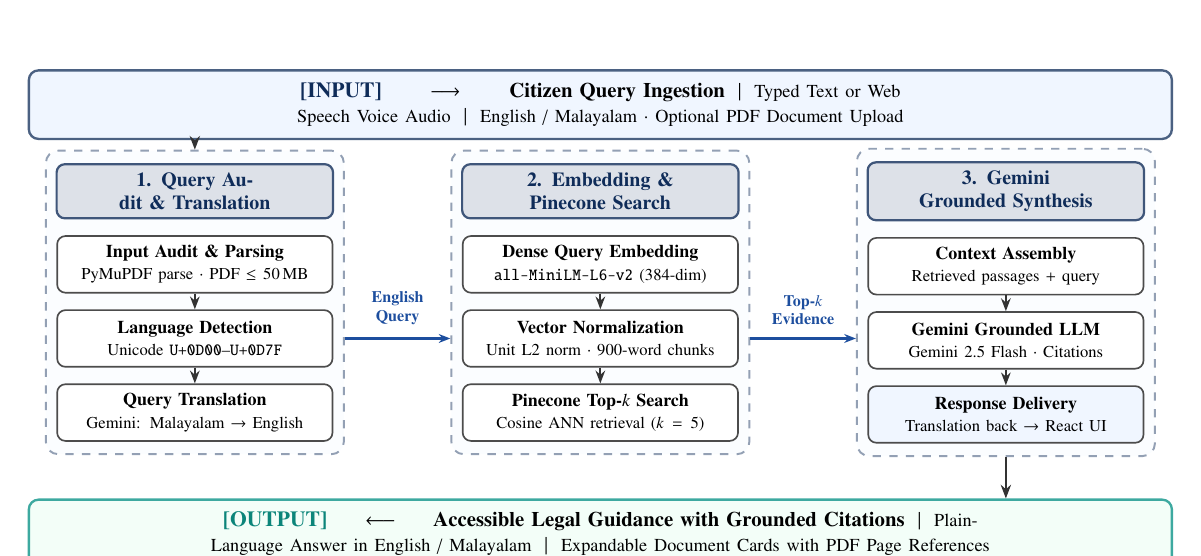
\begin{tikzpicture}[
    x=1cm, y=1cm,
    font=\sffamily,
    inout/.style={
        rectangle, rounded corners=3.5pt, line width=0.85pt,
        inner sep=4.5pt, align=center,
        font=\fontsize{7.5}{9.0}\selectfont
    },
    hdrbox/.style={
        rectangle, draw=lavenderDark!80, line width=0.80pt, fill=lavenderDark!14,
        rounded corners=3pt, inner sep=3.0pt, align=center,
        text width=3.30cm,
        font=\fontsize{7.2}{8.5}\selectfont\bfseries\color{lavenderDark}
    },
    stepbox/.style={
        rectangle, draw=black!70, line width=0.60pt, fill=white,
        rounded corners=3pt, inner sep=2.8pt, align=center,
        text width=3.30cm, minimum height=0.72cm,
        font=\fontsize{6.5}{7.6}\selectfont
    },
    stagebox/.style={
        rectangle, draw=lavenderDark!45, dashed, rounded corners=4.5pt, line width=0.70pt,
        fill=lavenderLight!25, inner xsep=3.5pt, inner ysep=4.5pt
    },
    flowarr/.style={
        -{Stealth[scale=0.75]}, line width=0.70pt, draw=black!80
    },
    transarr/.style={
        -{Stealth[length=4.2pt, width=3.2pt]}, line width=1.0pt, draw=lavenderMedium
    }
]

    % 1. TOP: INPUT BAR (width = 14.2cm)
    \node [inout, fill=lavenderLight, draw=lavenderDark!75, text width=14.2cm] (input_node) at (0, 3.60) {
        \textbf{\fontsize{7.8}{9.0}\selectfont\color{lavenderDark}[INPUT]} $\;\longrightarrow\;$
        \textbf{Citizen Query Ingestion}\; $\vert$\;
        {\fontsize{6.6}{7.8}\selectfont Typed Text or Web Speech Voice Audio}\; $\vert$\;
        {\fontsize{6.6}{7.8}\selectfont English / Malayalam $\cdot$ Optional PDF Document Upload}
    };

    % 2. MIDDLE: 3-STAGE HORIZONTAL PIPELINE
    % Spaced at x = -5.15, x = 0.00, x = +5.15 with text width = 3.30cm

    % --- STAGE 1: INGESTION & TRANSLATION (x = -5.15) ---
    \node [hdrbox] (h1) at (-5.15, 2.50) {1. Query Audit \& Translation};
    
    \node [stepbox, below=0.20cm of h1] (s1_1) {
        \textbf{Input Audit \& Parsing}\\[0.08em]
        {\fontsize{6.0}{7.0}\selectfont PyMuPDF parse $\cdot$ PDF $\le 50$\,MB}
    };
    \node [stepbox, below=0.20cm of s1_1] (s1_2) {
        \textbf{Language Detection}\\[0.08em]
        {\fontsize{6.0}{7.0}\selectfont Unicode \texttt{U+0D00}--\texttt{U+0D7F}}
    };
    \node [stepbox, below=0.20cm of s1_2] (s1_3) {
        \textbf{Query Translation}\\[0.08em]
        {\fontsize{6.0}{7.0}\selectfont Gemini: Malayalam $\to$ English}
    };

    \draw [flowarr] (s1_1) -- (s1_2);
    \draw [flowarr] (s1_2) -- (s1_3);

    \begin{scope}[on background layer]
    \node [stagebox, fit=(h1) (s1_3)] (stage1) {};
    \end{scope}

    % --- STAGE 2: EMBEDDING & RETRIEVAL (x = 0.00) ---
    \node [hdrbox] (h2) at (0.00, 2.50) {2. Embedding \& Pinecone Search};
    
    \node [stepbox, below=0.20cm of h2] (s2_1) {
        \textbf{Dense Query Embedding}\\[0.08em]
        {\fontsize{6.0}{7.0}\selectfont \texttt{all-MiniLM-L6-v2} (384-dim)}
    };
    \node [stepbox, below=0.20cm of s2_1] (s2_2) {
        \textbf{Vector Normalization}\\[0.08em]
        {\fontsize{6.0}{7.0}\selectfont Unit L2 norm $\cdot$ 900-word chunks}
    };
    \node [stepbox, below=0.20cm of s2_2] (s2_3) {
        \textbf{Pinecone Top-$k$ Search}\\[0.08em]
        {\fontsize{6.0}{7.0}\selectfont Cosine ANN retrieval ($k=5$)}
    };

    \draw [flowarr] (s2_1) -- (s2_2);
    \draw [flowarr] (s2_2) -- (s2_3);

    \begin{scope}[on background layer]
    \node [stagebox, fit=(h2) (s2_3)] (stage2) {};
    \end{scope}

    % --- STAGE 3: GENERATION & CITATIONS (x = +5.15) ---
    \node [hdrbox] (h3) at (5.15, 2.50) {3. Gemini Grounded Synthesis};
    
    \node [stepbox, below=0.20cm of h3] (s3_1) {
        \textbf{Context Assembly}\\[0.08em]
        {\fontsize{6.0}{7.0}\selectfont Retrieved passages + query}
    };
    \node [stepbox, below=0.20cm of s3_1] (s3_2) {
        \textbf{Gemini Grounded LLM}\\[0.08em]
        {\fontsize{6.0}{7.0}\selectfont Gemini 2.5 Flash $\cdot$ Citations}
    };
    \node [stepbox, below=0.20cm of s3_2, fill=lavenderLight] (s3_3) {
        \textbf{Response Delivery}\\[0.08em]
        {\fontsize{6.0}{7.0}\selectfont Translation back $\to$ React UI}
    };

    \draw [flowarr] (s3_1) -- (s3_2);
    \draw [flowarr] (s3_2) -- (s3_3);

    \begin{scope}[on background layer]
    \node [stagebox, fit=(h3) (s3_3)] (stage3) {};
    \end{scope}

    % Common elevation coordinate for perfectly horizontal inter-stage arrows
    \path let \p1 = (s1_2.center) in coordinate (transY) at (0, \y1);

    % Horizontal Transition Arrows in the Gap (2-line compact label, zero collision)
    \draw [transarr] (stage1.east |- transY) -- node[above=1pt, align=center, font=\fontsize{5.8}{6.8}\selectfont\bfseries\color{lavenderMedium}]{English\\Query} (stage2.west |- transY);
    \draw [transarr] (stage2.east |- transY) -- node[above=1pt, align=center, font=\fontsize{5.8}{6.8}\selectfont\bfseries\color{lavenderMedium}]{Top-$k$\\Evidence} (stage3.west |- transY);

    % Connect Top Input to Stage 1
    \draw [flowarr, line width=0.80pt] (input_node.south -| stage1.north) -- (stage1.north);

    % 3. BOTTOM: OUTPUT BAR (Positioned below stage boxes with 0.55cm clean margin)
    \node [inout, fill=prismMint!65, draw=prismTeal!80, text width=14.2cm, below=0.55cm of stage2] (output_node) {
        \textbf{\fontsize{7.8}{9.0}\selectfont\color{prismTeal!90!black}[OUTPUT]} $\;\longleftarrow\;$
        \textbf{Accessible Legal Guidance with Grounded Citations}\; $\vert$\;
        {\fontsize{6.6}{7.8}\selectfont Plain-Language Answer in English / Malayalam}\; $\vert$\;
        {\fontsize{6.6}{7.8}\selectfont Expandable Document Cards with PDF Page References}
    };

    % Connect Stage 3 to Output Bar
    \draw [flowarr, line width=0.80pt] (stage3.south) -- (output_node.north -| stage3.south);

\end{tikzpicture}
\end{document}
}
    \caption{Complete data flow from PDF upload through text extraction, chunking, embedding, and Pinecone indexing.}
    \label{fig:system_flow}
\end{figure}

\section{System Flowchart and Algorithms}

\subsection{System Flowchart}
Figure~\ref{fig:multiagent_flowchart} maps the decision pathways and exception branches executing during an inference request.

\begin{figure}[H]
    \centering
    \adjustbox{max width=0.98\linewidth, max height=0.72\textheight, keepaspectratio, center}{\documentclass[tikz,border=10pt]{standalone}
\usepackage{tikz}
\usepackage{fontawesome5}
\usepackage{amsmath,amssymb}
\usetikzlibrary{arrows.meta,positioning,fit,backgrounds,calc,shadows,shapes.geometric}

% Color definitions
\definecolor{lavenderDark}{RGB}{15, 44, 89}
\definecolor{lavenderDeep}{RGB}{10, 28, 58}
\definecolor{lavenderMedium}{RGB}{29, 78, 158}
\definecolor{lavenderLight}{RGB}{240, 246, 255}
\definecolor{lavenderBorder}{RGB}{180, 205, 237}
\definecolor{prismNavy}{RGB}{15, 44, 89}
\definecolor{prismBlue}{RGB}{29, 78, 158}
\definecolor{prismTeal}{RGB}{13, 148, 136}
\definecolor{prismGold}{RGB}{217, 119, 6}
\definecolor{prismDark}{RGB}{15, 23, 42}
\definecolor{statusFail}{RGB}{220, 38, 38}
\definecolor{cInput}{RGB}{241, 245, 249}
\definecolor{cStem}{RGB}{224, 242, 254}
\definecolor{cStage1}{RGB}{209, 250, 229}
\definecolor{cStage2}{RGB}{254, 243, 199}
\definecolor{cHead}{RGB}{219, 234, 254}

\begin{document}
% Complete Flowchart for CiviQ Legal RAG Query Processing & Translation
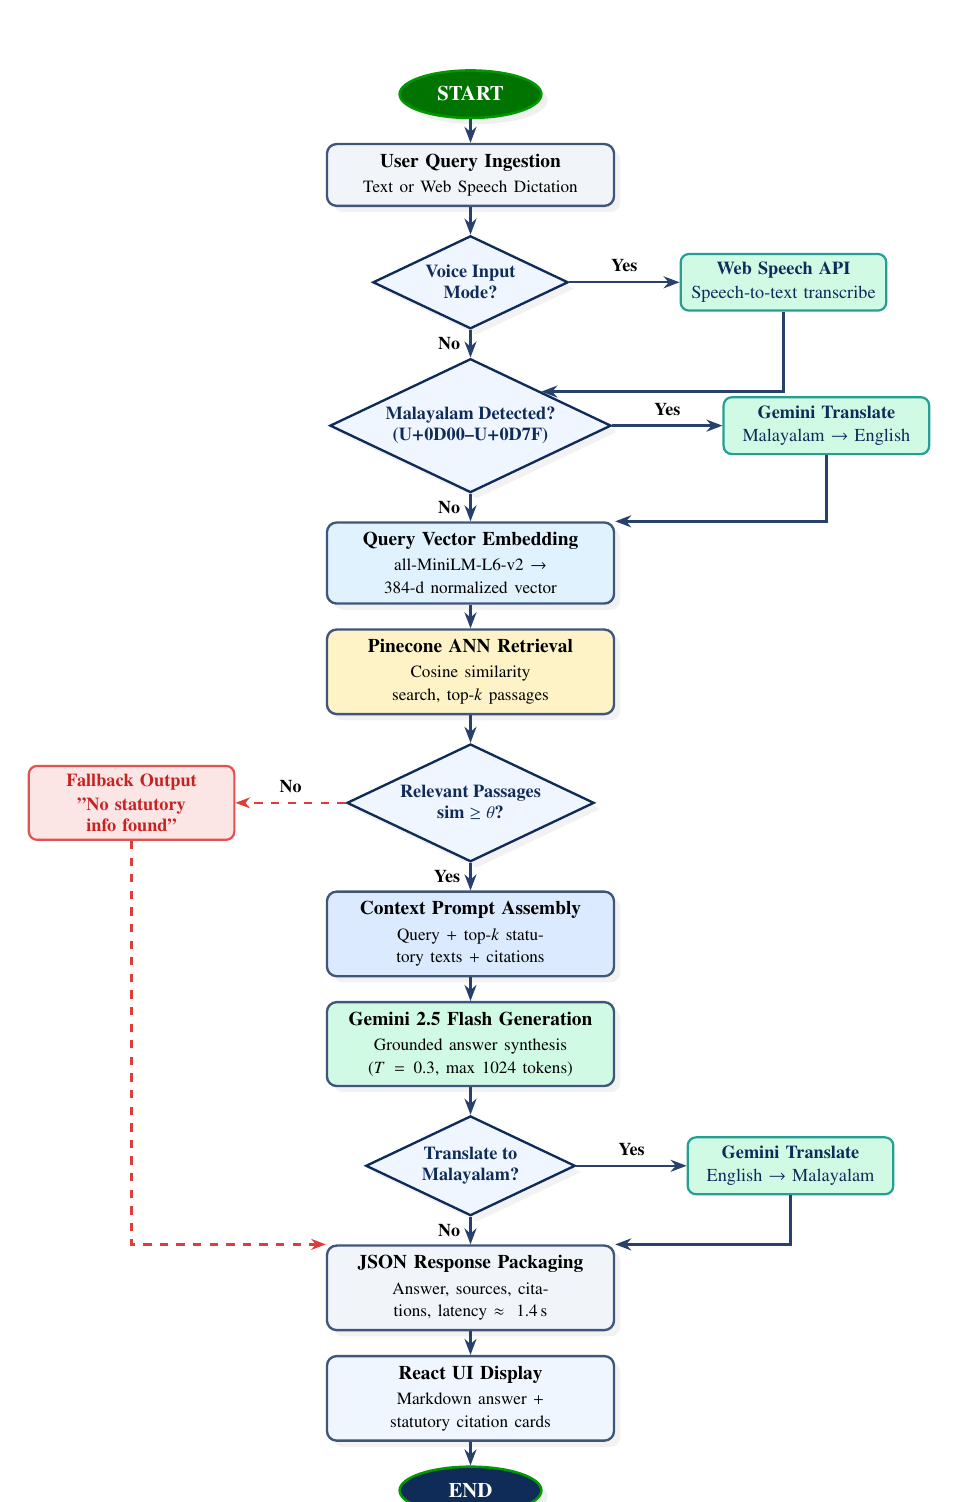
\begin{tikzpicture}[
  x=1cm, y=1cm,
  font=\sffamily,
  startend/.style={
    ellipse, draw=green!60!black, fill=green!45!black, text=white,
    line width=0.9pt, inner sep=3.5pt, font=\fontsize{7.5}{8.5}\selectfont\bfseries,
    minimum width=1.80cm, minimum height=0.60cm, drop shadow={opacity=0.12}
  },
  procbox/.style={
    rectangle, rounded corners=3.5pt,
    draw=lavenderDark!80, fill=white, text=black,
    line width=0.85pt, inner sep=3.5pt, font=\fontsize{7.0}{8.2}\selectfont,
    minimum height=0.68cm, text width=3.40cm, align=center, drop shadow={opacity=0.10}
  },
  decision/.style={
    diamond, aspect=2.1,
    draw=prismNavy, fill=lavenderLight, text=prismNavy,
    line width=0.85pt, inner sep=2.0pt, font=\fontsize{6.6}{7.6}\selectfont\bfseries,
    align=center, drop shadow={opacity=0.10}
  },
  sidebox/.style={
    rectangle, rounded corners=3pt,
    draw=prismTeal!90, fill=cStage1, text=prismNavy,
    line width=0.80pt, inner sep=3.0pt, font=\fontsize{6.6}{7.6}\selectfont,
    minimum height=0.60cm, text width=2.40cm, align=center
  },
  errorbox/.style={
    rectangle, rounded corners=3pt,
    draw=statusFail!80, fill=statusFail!12, text=statusFail!90!black,
    line width=0.80pt, inner sep=3.0pt, font=\fontsize{6.6}{7.6}\selectfont\bfseries,
    minimum height=0.60cm, text width=2.40cm, align=center
  },
  flowarr/.style={
    -{Stealth[scale=0.85]}, line width=0.85pt, draw=lavenderDark!90
  },
  failarr/.style={
    -{Stealth[scale=0.80]}, line width=0.80pt, draw=statusFail!90, dashed
  }
]

  % Central Column - Main Processing Flow
  \node[startend] (start) at (0, 11.20) {START};

  \node[procbox, fill=cInput, below=0.30cm of start] (user_in) {%
    \textbf{User Query Ingestion}\\[1pt]
    {\fontsize{6.2}{7.2}\selectfont Text or Web Speech Dictation}%
  };

  \node[decision, below=0.35cm of user_in] (d_voice) {%
    Voice Input\\Mode?%
  };

  \node[decision, below=0.35cm of d_voice] (d_lang) {%
    Malayalam Detected?\\(U+0D00--U+0D7F)%
  };

  \node[procbox, fill=cStem, below=0.35cm of d_lang] (embed) {%
    \textbf{Query Vector Embedding}\\[1pt]
    {\fontsize{6.2}{7.2}\selectfont all-MiniLM-L6-v2 $\to$ 384-d normalized vector}%
  };

  \node[procbox, fill=cStage2, below=0.30cm of embed] (pinecone) {%
    \textbf{Pinecone ANN Retrieval}\\[1pt]
    {\fontsize{6.2}{7.2}\selectfont Cosine similarity search, top-$k$ passages}%
  };

  \node[decision, below=0.35cm of pinecone] (d_match) {%
    Relevant Passages\\$\text{sim} \ge \theta$?%
  };

  \node[procbox, fill=cHead, below=0.35cm of d_match] (prompt_bld) {%
    \textbf{Context Prompt Assembly}\\[1pt]
    {\fontsize{6.2}{7.2}\selectfont Query + top-$k$ statutory texts + citations}%
  };

  \node[procbox, fill=cStage1, below=0.30cm of prompt_bld] (gemini) {%
    \textbf{Gemini 2.5 Flash Generation}\\[1pt]
    {\fontsize{6.2}{7.2}\selectfont Grounded answer synthesis ($T=0.3$, max 1024 tokens)}%
  };

  \node[decision, below=0.35cm of gemini] (d_trans_back) {%
    Translate to\\Malayalam?%
  };

  \node[procbox, fill=cInput, below=0.35cm of d_trans_back] (respond) {%
    \textbf{JSON Response Packaging}\\[1pt]
    {\fontsize{6.2}{7.2}\selectfont Answer, sources, citations, latency $\approx 1.4$\,s}%
  };

  \node[procbox, fill=lavenderLight, below=0.30cm of respond] (render) {%
    \textbf{React UI Display}\\[1pt]
    {\fontsize{6.2}{7.2}\selectfont Markdown answer + statutory citation cards}%
  };

  \node[startend, fill=lavenderDark, below=0.30cm of render] (end) {END};

  % Side Branches (Left/Right)
  % 1. Voice transcription (Right of d_voice)
  \node[sidebox, right=1.40cm of d_voice] (voice_stt) {%
    \textbf{Web Speech API}\\[1pt]
    Speech-to-text transcribe%
  };

  % 2. Translation to English (Right of d_lang)
  \node[sidebox, right=1.40cm of d_lang] (trans_en) {%
    \textbf{Gemini Translate}\\[1pt]
    Malayalam $\to$ English%
  };

  % 3. No match error (Left of d_match)
  \node[errorbox, left=1.40cm of d_match] (no_match) {%
    \textbf{Fallback Output}\\[1pt]
    "No statutory info found"%
  };

  % 4. Translation to Malayalam (Right of d_trans_back)
  \node[sidebox, right=1.40cm of d_trans_back] (trans_ml) {%
    \textbf{Gemini Translate}\\[1pt]
    English $\to$ Malayalam%
  };

  % Downward Connections
  \draw[flowarr] (start) -- (user_in);
  \draw[flowarr] (user_in) -- (d_voice);
  \draw[flowarr] (d_voice) -- node[left, font=\fontsize{6.5}{7.5}\selectfont\bfseries]{No} (d_lang);
  \draw[flowarr] (d_lang) -- node[left, font=\fontsize{6.5}{7.5}\selectfont\bfseries]{No} (embed);
  \draw[flowarr] (embed) -- (pinecone);
  \draw[flowarr] (pinecone) -- (d_match);
  \draw[flowarr] (d_match) -- node[left, font=\fontsize{6.5}{7.5}\selectfont\bfseries]{Yes} (prompt_bld);
  \draw[flowarr] (prompt_bld) -- (gemini);
  \draw[flowarr] (gemini) -- (d_trans_back);
  \draw[flowarr] (d_trans_back) -- node[left, font=\fontsize{6.5}{7.5}\selectfont\bfseries]{No} (respond);
  \draw[flowarr] (respond) -- (render);
  \draw[flowarr] (render) -- (end);

  % Branch: Voice transcription
  \draw[flowarr] (d_voice.east) -- node[above, font=\fontsize{6.5}{7.5}\selectfont\bfseries]{Yes} (voice_stt.west);
  \draw[flowarr] (voice_stt.south) |- (d_lang.north east);

  % Branch: Translation to English
  \draw[flowarr] (d_lang.east) -- node[above, font=\fontsize{6.5}{7.5}\selectfont\bfseries]{Yes} (trans_en.west);
  \draw[flowarr] (trans_en.south) |- (embed.north east);

  % Branch: Fallback when no match
  \draw[failarr] (d_match.west) -- node[above, font=\fontsize{6.5}{7.5}\selectfont\bfseries]{No} (no_match.east);
  \draw[failarr] (no_match.south) |- (respond.north west);

  % Branch: Translation to Malayalam
  \draw[flowarr] (d_trans_back.east) -- node[above, font=\fontsize{6.5}{7.5}\selectfont\bfseries]{Yes} (trans_ml.west);
  \draw[flowarr] (trans_ml.south) |- (respond.north east);

\end{tikzpicture}
\end{document}
}
    \caption{Query processing flowchart with decision branches for language detection, retrieval depth, and error handling.}
    \label{fig:multiagent_flowchart}
\end{figure}

\subsection{Algorithm}
The complete operational algorithm governing RAG ingestion, query processing, and answer generation is formalized below across ten sequential operational steps:

\subsubsection*{Step 1: PDF Document Acquisition and Validation}
\begin{enumerate}
  \item[\textbf{1.1}] Ingest PDF document $\mathcal{D}_{\text{in}}$ via HTTP multipart form upload.
  \item[\textbf{1.2}] Perform MIME header verification: $\mathrm{MIME} = \texttt{application/pdf}$.
  \item[\textbf{1.3}] Enforce payload boundary limit: Verify $\mathrm{size}(\mathcal{D}_{\text{in}}) \le 50\,\mathrm{MB}$; return HTTP 413 on violation.
  \item[\textbf{1.4}] Execute PyMuPDF integrity check and extract page count.
\end{enumerate}

\subsubsection*{Step 2: Text Extraction and Cleaning}
\begin{enumerate}
  \item[\textbf{2.1}] Extract text from each PDF page using PyMuPDF (fitz): $T = \bigcup_{p=1}^{N} \text{extract\_text}(p)$.
  \item[\textbf{2.2}] Remove header artifacts (page numbers, footers) using regex pattern matching.
  \item[\textbf{2.3}] Normalize whitespace: collapse multiple spaces, remove zero-width characters.
\end{enumerate}

\subsubsection*{Step 3: Overlapping Word-Chunking}
\begin{enumerate}
  \item[\textbf{3.1}] Split cleaned text $T$ into word tokens: $W = [w_1, w_2, \dots, w_M]$.
  \item[\textbf{3.2}] Create overlapping chunks with size $c = 900$ words, stride $s = 750$ words (overlap 150):
    \begin{equation}
      \text{chunk}_i = W[i \cdot s : i \cdot s + c]
    \end{equation}
  \item[\textbf{3.3}] Filter chunks shorter than 40 words to discard artifacts.
\end{enumerate}

\subsubsection*{Step 4: Sentence-Transformer Embedding}
\begin{enumerate}
  \item[\textbf{4.1}] Load all-MiniLM-L6-v2 model: $\phi: \mathcal{T} \to \mathbb{R}^{384}$.
  \item[\textbf{4.2}] Embed each chunk: $\mathbf{e}_i = \phi(\text{chunk}_i)$.
  \item[\textbf{4.3}] Apply L2 normalization:
    \begin{equation}
      \mathbf{e}_i^{\text{norm}} = \frac{\mathbf{e}_i}{\|\mathbf{e}_i\|_2}
    \end{equation}
\end{enumerate}

\subsubsection*{Step 5: Pinecone Vector Database Upsert}
\begin{enumerate}
  \item[\textbf{5.1}] Prepare batch upsert payload: group embeddings into batches of 100 vectors.
  \item[\textbf{5.2}] Construct metadata: $\{\text{doc\_name}, \text{chunk\_index}, \text{chunk\_text}\}$.
  \item[\textbf{5.3}] Upsert to Pinecone namespace with unique IDs and cosine similarity metric.
\end{enumerate}

\subsubsection*{Step 6: User Query Ingestion and Language Detection}
\begin{enumerate}
  \item[\textbf{6.1}] Accept user query $q$ via text input or Web Speech API voice transcription.
  \item[\textbf{6.2}] Detect Malayalam: check if any character $c \in q$ satisfies $\texttt{U+0D00} \le c \le \texttt{U+0D7F}$.
  \item[\textbf{6.3}] If Malayalam detected, translate to English: $q_{\text{en}} = \text{Gemini\_Translate}(q_{\text{ml}})$.
\end{enumerate}

\subsubsection*{Step 7: Query Embedding and Semantic Retrieval}
\begin{enumerate}
  \item[\textbf{7.1}] Embed query using identical model: $\mathbf{e}_q = \phi(q_{\text{en}})$ and normalize.
  \item[\textbf{7.2}] Query Pinecone with top-k parameter (default k=5):
    \begin{equation}
      R = \text{Pinecone.query}(\mathbf{e}_q, \text{top\_k}=k)
    \end{equation}
  \item[\textbf{7.3}] Retrieve passages with similarity scores: $\{(p_1, s_1), (p_2, s_2), \dots, (p_k, s_k)\}$.
\end{enumerate}

\subsubsection*{Step 8: Context Assembly and Prompt Construction}
\begin{enumerate}
  \item[\textbf{8.1}] Concatenate retrieved passages: $\text{context} = \bigcup_{i=1}^k p_i$.
  \item[\textbf{8.2}] Construct Gemini prompt template:
    \begin{verbatim}
    You are a legal information assistant. Answer based 
    ONLY on provided context. Question: {q}. 
    Context: {context}. Cite specific sections/acts.
    \end{verbatim}
\end{enumerate}

\subsubsection*{Step 9: Gemini Answer Generation with Citations}
\begin{enumerate}
  \item[\textbf{9.1}] Call Gemini 2.5 Flash API with temperature=0.3, max\_output\_tokens=1024.
  \item[\textbf{9.2}] Extract answer text and parse source citations (Act names, section numbers).
  \item[\textbf{9.3}] If original query was Malayalam, translate answer: $\text{answer}_{\text{ml}} = \text{Gemini\_Translate}(\text{answer}_{\text{en}})$.
\end{enumerate}

\subsubsection*{Step 10: Response Formatting and Delivery}
\begin{enumerate}
  \item[\textbf{10.1}] Format JSON response: $\{\text{answer}, \text{sources}[], \text{language}, \text{latency}\}$.
  \item[\textbf{10.2}] Return HTTP 200 with response body to frontend.
  \item[\textbf{10.3}] Frontend renders answer with Markdown and displays source citation cards.
\end{enumerate}

\subsection{RAG Pipeline Component Dependencies}
Figure~\ref{fig:dag_scheduling_walkthrough} illustrates the component dependencies in the RAG ingestion and query pipeline. The directed acyclic execution graph traces the transformation of raw PDF legal statutes into cleaned, normalized text chunks, followed by embedding generation and Pinecone vector upload. Query execution parallels this workflow: incoming text or voice queries are embedded with the identical transformer encoder, enabling cosine distance comparison against the pre-indexed legal corpus, subsequent context compilation, and Gemini-based synthesis.

\begin{figure}[H]
    \centering
    \adjustbox{max width=0.98\linewidth, max height=0.68\textheight, keepaspectratio, center}{\documentclass[tikz,border=10pt]{standalone}
\usepackage{tikz}
\usepackage{fontawesome5}
\usepackage{amsmath,amssymb}
\usetikzlibrary{arrows.meta,positioning,fit,backgrounds,calc,shadows,shapes.geometric}

% Color definitions
\definecolor{lavenderDark}{RGB}{15, 44, 89}
\definecolor{lavenderDeep}{RGB}{10, 28, 58}
\definecolor{lavenderMedium}{RGB}{29, 78, 158}
\definecolor{lavenderLight}{RGB}{240, 246, 255}
\definecolor{lavenderBorder}{RGB}{180, 205, 237}
\definecolor{prismNavy}{RGB}{15, 44, 89}
\definecolor{prismBlue}{RGB}{29, 78, 158}
\definecolor{prismTeal}{RGB}{13, 148, 136}
\definecolor{prismMint}{RGB}{236, 253, 245}
\definecolor{prismGold}{RGB}{217, 119, 6}
\definecolor{prismDark}{RGB}{15, 23, 42}
\definecolor{prismSlate}{RGB}{100, 116, 139}
\definecolor{cInput}{RGB}{241, 245, 249}
\definecolor{cStem}{RGB}{224, 242, 254}
\definecolor{cStage1}{RGB}{209, 250, 229}
\definecolor{cStage2}{RGB}{254, 243, 199}
\definecolor{cStage3}{RGB}{254, 226, 226}
\definecolor{cStage4}{RGB}{207, 250, 254}

\begin{document}
% RAG Pipeline Component Dependencies and Execution DAG
\begin{tikzpicture}[
  x=1cm, y=1cm,
  font=\sffamily,
  dagstep/.style={
    rectangle, rounded corners=3.5pt, minimum height=1.00cm,
    text width=2.90cm, align=center, draw=lavenderDark!75, fill=lavenderLight!85,
    line width=0.85pt, font=\fontsize{7.5}{8.8}\selectfont\bfseries,
    drop shadow={shadow xshift=0.8pt, shadow yshift=-0.8pt, opacity=0.10}
  },
  dagarrow/.style={-{Stealth[length=4.0pt, width=3.0pt]}, line width=0.95pt, draw=prismTeal!95!black},
  dagnode/.style={
    rectangle, rounded corners=3.5pt, line width=0.75pt,
    minimum height=1.15cm, text width=1.65cm, inner sep=2.5pt, align=center,
    font=\fontsize{6.2}{7.3}\selectfont,
    drop shadow={shadow xshift=0.6pt, shadow yshift=-0.6pt, opacity=0.08}
  },
  idxnode/.style={
    cylinder, shape border rotate=90, aspect=0.25, line width=0.85pt,
    draw=prismTeal!95!black, fill=prismMint, minimum height=1.30cm, text width=1.60cm, inner sep=2.0pt, align=center,
    font=\fontsize{6.5}{7.5}\selectfont\bfseries,
    drop shadow={shadow xshift=0.6pt, shadow yshift=-0.6pt, opacity=0.12}
  },
  loopconn/.style={-{Stealth[length=4.0pt, width=3.0pt]}, line width=0.85pt, draw=lavenderDark!80, dashed}
]

  % Row 1: 4-Stage Architectural Overview (Centers: -5.40, -1.80, 1.80, 5.40)
  \node[dagstep] (s1) at (-5.40, 0) {1. Corpus Preprocessing\\[2pt]\normalfont\fontsize{6.5}{7.5}\selectfont PyMuPDF Extraction $\to$ Cleaning\\[1pt]900-word Chunks ($o=150$)};
  \node[dagstep] (s2) at (-1.80, 0) {2. Vector Ingestion\\[2pt]\normalfont\fontsize{6.5}{7.5}\selectfont all-MiniLM-L6-v2 ($384$-d)\\[1pt]Pinecone Cosine Index};
  \node[dagstep] (s3) at (1.80, 0) {3. Semantic Retrieval\\[2pt]\normalfont\fontsize{6.5}{7.5}\selectfont Query Embedding $\to$ Cosine ANN\\[1pt]Top-$k$ Statutory Passages};
  \node[dagstep] (s4) at (5.40, 0) {4. Grounded Synthesis\\[2pt]\normalfont\fontsize{6.5}{7.5}\selectfont Gemini 2.5 Flash ($T=0.3$)\\[1pt]Citation Grounding \& Translation};

  \draw[dagarrow] (s1) -- (s2);
  \draw[dagarrow] (s2) -- (s3);
  \draw[dagarrow] (s3) -- (s4);

  % Separator line
  \draw[draw=lavenderBorder, line width=0.6pt] (-8.0, -0.90) -- (8.0, -0.90);

  % Section Header A
  \node[anchor=west, font=\fontsize{6.8}{8.0}\selectfont\bfseries\color{lavenderDark}] at (-7.9, -1.30) {\faCogs\ Offline Corpus Ingestion Pipeline};

  % ================= PIPELINE A: STATUTE INGESTION DAG (Row 2: y = -2.35) =================
  % Centers at x = -7.00, -4.60, -2.20, +0.20, +2.60, +5.00
  \node[dagnode, fill=cInput, draw=prismSlate!80] (pdf_in) at (-7.00, -2.35) {
    \textbf{\faFilePdf\ PDF Corpus}\\[1.5pt]
    {\fontsize{5.5}{6.5}\selectfont BNS, BNSS, BSA,\\[0.5pt]RTI, Consumer}
  };

  \node[dagnode, fill=cStem, draw=lavenderDark] (mupdf) at (-4.60, -2.35) {
    \textbf{\faSearch\ PyMuPDF}\\[1.5pt]
    {\fontsize{5.5}{6.5}\selectfont Stream extraction\\[0.5pt]\& page parsing}
  };

  \node[dagnode, fill=cStage1, draw=prismTeal] (clean) at (-2.20, -2.35) {
    \textbf{\faBroom\ Text Cleaner}\\[1.5pt]
    {\fontsize{5.5}{6.5}\selectfont Strip headers,\\[0.5pt]footers \& noise}
  };

  \node[dagnode, fill=cStage2, draw=prismGold!90] (chunk) at (0.20, -2.35) {
    \textbf{\faCut\ Word Chunker}\\[1.5pt]
    {\fontsize{5.5}{6.5}\selectfont $c=900, o=150$\\[0.5pt]min 40 words}
  };

  \node[dagnode, fill=cStage4, draw=prismBlue!90] (embed) at (2.60, -2.35) {
    \textbf{\faBrain\ MiniLM-L6-v2}\\[1.5pt]
    {\fontsize{5.5}{6.5}\selectfont 384-d dense vector\\[0.5pt]L2-normalized}
  };

  \node[dagnode, fill=cStage1, draw=lavenderMedium] (batch) at (5.00, -2.35) {
    \textbf{\faBoxes\ Batch Loader}\\[1.5pt]
    {\fontsize{5.5}{6.5}\selectfont Batch size: 100\\[0.5pt]Metadata injection}
  };

  % Ingestion forward edges with clear gaps
  \draw[dagarrow] (pdf_in) -- (mupdf);
  \draw[dagarrow] (mupdf) -- (clean);
  \draw[dagarrow] (clean) -- (chunk);
  \draw[dagarrow] (chunk) -- (embed);
  \draw[dagarrow] (embed) -- (batch);

  % ================= CENTRAL DATASTORE: PINECONE VECTOR INDEX (y = -3.85) =================
  \node[idxnode] (pinecone) at (7.15, -3.85) {
    \faDatabase\ \textbf{Pinecone}\\[1.5pt]
    \normalfont{\fontsize{5.5}{6.5}\selectfont HNSW Index\\[0.5pt]Cosine Metric}
  };

  \draw[dagarrow] (batch.east) to[out=0, in=90] (pinecone.north);

  % Section Header B
  \node[anchor=west, font=\fontsize{6.8}{8.0}\selectfont\bfseries\color{lavenderDark}] at (-7.9, -4.35) {\faBolt\ Online Query Processing \& Grounded Synthesis};

  % ================= PIPELINE B: QUERY & SYNTHESIS DAG (Row 3: y = -5.40) =================
  \node[dagnode, fill=cInput, draw=prismSlate!80] (query_in) at (-7.00, -5.40) {
    \textbf{\faUser\ User Query}\\[1.5pt]
    {\fontsize{5.5}{6.5}\selectfont Text input /\\[0.5pt]Speech Audio}
  };

  \node[dagnode, fill=cStem, draw=lavenderDark] (lang_router) at (-4.60, -5.40) {
    \textbf{\faLanguage\ Lang Router}\\[1.5pt]
    {\fontsize{5.5}{6.5}\selectfont Unicode check\\[0.5pt]Malayalam $\to$ En}
  };

  \node[dagnode, fill=cStage4, draw=prismBlue!90] (q_embed) at (-2.20, -5.40) {
    \textbf{\faBrain\ Query Embed}\\[1.5pt]
    {\fontsize{5.5}{6.5}\selectfont MiniLM-L6-v2\\[0.5pt]384-d normalized}
  };

  \node[dagnode, fill=cStage2, draw=prismGold!90] (q_retrieve) at (0.20, -5.40) {
    \textbf{\faSearchPlus\ Top-$k$ Retriever}\\[1.5pt]
    {\fontsize{5.5}{6.5}\selectfont Cosine ANN\\[0.5pt]Top-$k$ ($k=5$)}
  };

  \node[dagnode, fill=cStage3, draw=prismNavy] (llm_gen) at (2.60, -5.40) {
    \textbf{\faRobot\ Gemini 2.5 Flash}\\[1.5pt]
    {\fontsize{5.5}{6.5}\selectfont Grounded LLM\\[0.5pt]Context prompt}
  };

  \node[dagnode, fill=cStage1, draw=prismTeal] (response_out) at (5.00, -5.40) {
    \textbf{\faCheckCircle\ Final Delivery}\\[1.5pt]
    {\fontsize{5.5}{6.5}\selectfont Citations + UI\\[0.5pt]$\approx 1.4$\,s latency}
  };

  % Query execution forward edges with clear gaps
  \draw[dagarrow] (query_in) -- (lang_router);
  \draw[dagarrow] (lang_router) -- (q_embed);
  \draw[dagarrow] (q_embed) -- (q_retrieve);
  \draw[dagarrow] (q_retrieve) -- (llm_gen);
  \draw[dagarrow] (llm_gen) -- (response_out);

  % Pinecone interaction edge
  \draw[dagarrow, dashed, draw=prismTeal!95!black] (pinecone.west) to[out=180, in=60] 
    node[above=1pt, font=\fontsize{5.6}{6.6}\selectfont\color{prismTeal!90!black}]{Passage vectors} (q_retrieve.north);

  % User feedback / query refinement loop
  \draw[loopconn] (response_out.south) to[out=270, in=270, looseness=0.42] 
    node[below=2pt, font=\fontsize{6.2}{7.2}\selectfont\bfseries\color{lavenderDark}]{Iterative Refinement / Follow-up Inquiry} 
    (query_in.south);

\end{tikzpicture}
\end{document}
}
    \caption{RAG pipeline component dependencies: PyMuPDF $\to$ text cleaner $\to$ chunker $\to$ embedder $\to$ Pinecone uploader.}
    \label{fig:dag_scheduling_walkthrough}
\end{figure}

\section{Detailed Component Analysis}

\subsection{Data Storage, Model Artifacts, and Schema Connectors}
Figure~\ref{fig:db_schema} depicts the relational schema architecture connecting legal document metadata, text chunks, vector embeddings, retrieval configuration parameters, query logs, and response records.

\begin{figure}[H]
    \centering
    \adjustbox{max width=0.98\linewidth, max height=0.72\textheight, keepaspectratio, center}{\documentclass[tikz,border=10pt]{standalone}
\usepackage{tikz}
\usepackage{fontawesome5}
\usepackage{amsmath,amssymb}
\usetikzlibrary{arrows.meta,positioning,fit,backgrounds,calc,shadows,shapes.geometric}

% Color definitions
\definecolor{lavenderDark}{RGB}{15, 44, 89}
\definecolor{lavenderDeep}{RGB}{10, 28, 58}
\definecolor{lavenderMedium}{RGB}{29, 78, 158}
\definecolor{lavenderLight}{RGB}{240, 246, 255}
\definecolor{lavenderBorder}{RGB}{180, 205, 237}
\definecolor{prismTeal}{RGB}{13, 148, 136}
\definecolor{prismMint}{RGB}{236, 253, 245}
\definecolor{prismGold}{RGB}{217, 119, 6}
\definecolor{prismDark}{RGB}{15, 23, 42}

\begin{document}
% Relational Entity & Storage Schema Connectors for CiviQ Legal RAG System
\begin{tikzpicture}[
  x=1cm, y=1cm,
  font=\sffamily,
  tblcard/.style={
    rectangle, rounded corners=4pt, draw=lavenderDark!75, line width=0.85pt, fill=white,
    inner sep=5pt, text width=4.30cm, align=left,
    drop shadow={shadow xshift=1pt, shadow yshift=-1pt, opacity=0.12}
  },
  fkarrow/.style={
    -{Stealth[scale=0.85]}, line width=1.0pt, draw=lavenderDark!90
  },
  fklabel/.style={
    font=\fontsize{6.0}{7.0}\selectfont\bfseries, fill=white, inner sep=1.2pt, text=lavenderDark
  }
]

  % ================= COLUMN 1: CORPUS & CHUNKS (x = -5.2) =================
  
  % Table 1: document_corpus_store
  \node[tblcard] (corpus) at (-5.2, 2.5) {%
    \centerline{\color{lavenderDark}\faBook\ \textbf{\fontsize{8.0}{9.5}\selectfont document\_corpus\_store}}\\[3pt]
    \rule{\linewidth}{0.4pt}\\[3pt]
    {\fontsize{6.6}{7.8}\selectfont
    \textbf{\color{lavenderDark}[PK]} \texttt{doc\_id}: \textit{string} (UUID / Hash)\\
    \textbf{\color{prismTeal}[FLD]} \texttt{filename}: \textit{string} (\texttt{bns.pdf}, \texttt{rti.pdf})\\
    \textbf{\color{prismDark!80}[FLD]} \texttt{statute\_title}: \textit{BNS 2023, RTI Act 2005}\\
    \textbf{\color{prismDark!80}[FLD]} \texttt{page\_count}: \textit{integer} (Total pages)\\
    \textbf{\color{prismDark!80}[FLD]} \texttt{checksum}: \textit{SHA-256 integrity tag}}%
  };

  % Table 2: chunk_store
  \node[tblcard, below=0.70cm of corpus] (chunk) {%
    \centerline{\color{lavenderDark}\faStream\ \textbf{\fontsize{8.0}{9.5}\selectfont chunk\_store}}\\[3pt]
    \rule{\linewidth}{0.4pt}\\[3pt]
    {\fontsize{6.6}{7.8}\selectfont
    \textbf{\color{lavenderDark}[PK]} \texttt{chunk\_id}: \textit{string} (\texttt{doc\_id\_pX\_cY})\\
    \textbf{\color{prismTeal}[FK]} \texttt{doc\_id}: \textit{corpus reference}\\
    \textbf{\color{prismDark!80}[FLD]} \texttt{page\_number}: \textit{integer} (PDF source page)\\
    \textbf{\color{prismDark!80}[FLD]} \texttt{chunk\_text}: \textit{text} ($c=900$ words)\\
    \textbf{\color{prismDark!80}[FLD]} \texttt{overlap\_words}: \textit{integer} ($o=150$)\\
    \textbf{\color{prismDark!80}[FLD]} \texttt{token\_count}: \textit{integer} ($\ge 40$ words)}%
  };

  % ================= COLUMN 2: VECTOR EMBEDDINGS & RETRIEVAL (x = 0) =================
  
  % Table 3: vector_embeddings_store
  \node[tblcard] (vector) at (0, 2.5) {%
    \centerline{\color{lavenderDark}\faDatabase\ \textbf{\fontsize{8.0}{9.5}\selectfont vector\_embeddings\_store}}\\[3pt]
    \rule{\linewidth}{0.4pt}\\[3pt]
    {\fontsize{6.6}{7.8}\selectfont
    \textbf{\color{lavenderDark}[PK]} \texttt{vector\_id}: \textit{string} (Pinecone ID)\\
    \textbf{\color{prismTeal}[FK]} \texttt{chunk\_id}: \textit{chunk reference}\\
    \textbf{\color{prismDark!80}[FLD]} \texttt{embedding}: \textit{float[384]} (L2-normalized)\\
    \textbf{\color{prismDark!80}[FLD]} \texttt{model}: \textit{all-MiniLM-L6-v2}\\
    \textbf{\color{prismDark!80}[FLD]} \texttt{namespace}: \textit{legal-statutes-2023}\\
    \textbf{\color{prismDark!80}[FLD]} \texttt{indexed\_at}: \textit{timestamp}}%
  };

  % Table 4: retrieval_config_store
  \node[tblcard, below=0.70cm of vector] (config) {%
    \centerline{\color{lavenderDark}\faSlidersH\ \textbf{\fontsize{8.0}{9.5}\selectfont retrieval\_config\_store}}\\[3pt]
    \rule{\linewidth}{0.4pt}\\[3pt]
    {\fontsize{6.6}{7.8}\selectfont
    \textbf{\color{lavenderDark}[PK]} \texttt{config\_id}: \textit{string} (Preset ID)\\
    \textbf{\color{prismDark!80}[FLD]} \texttt{top\_k}: \textit{integer} ($k=5$, range $1\dots 10$)\\
    \textbf{\color{prismDark!80}[FLD]} \texttt{metric}: \textit{cosine similarity}\\
    \textbf{\color{prismDark!80}[FLD]} \texttt{min\_similarity}: \textit{float} ($\theta \ge 0.45$)\\
    \textbf{\color{prismDark!80}[FLD]} \texttt{temperature}: \textit{0.3} (LLM determinism)\\
    \textbf{\color{prismDark!80}[FLD]} \texttt{max\_tokens}: \textit{1024 output tokens}}%
  };

  % ================= COLUMN 3: QUERY LOGS & RESPONSES (x = 5.2) =================
  
  % Table 5: query_log_store
  \node[tblcard] (query) at (5.2, 2.5) {%
    \centerline{\color{lavenderDark}\faComments\ \textbf{\fontsize{8.0}{9.5}\selectfont query\_log\_store}}\\[3pt]
    \rule{\linewidth}{0.4pt}\\[3pt]
    {\fontsize{6.6}{7.8}\selectfont
    \textbf{\color{lavenderDark}[PK]} \texttt{query\_id}: \textit{UUID}\\
    \textbf{\color{prismTeal}[FK]} \texttt{config\_id}: \textit{retrieval config}\\
    \textbf{\color{prismDark!80}[FLD]} \texttt{raw\_query}: \textit{text} (User prompt)\\
    \textbf{\color{prismDark!80}[FLD]} \texttt{input\_channel}: \textit{text / WebSpeech voice}\\
    \textbf{\color{prismDark!80}[FLD]} \texttt{detected\_lang}: \textit{en / ml}\\
    \textbf{\color{prismDark!80}[FLD]} \texttt{translated\_query}: \textit{text (if ml)}}%
  };

  % Table 6: response_log_store
  \node[tblcard, below=0.70cm of query] (response) {%
    \centerline{\color{lavenderDark}\faFileContract\ \textbf{\fontsize{8.0}{9.5}\selectfont response\_log\_store}}\\[3pt]
    \rule{\linewidth}{0.4pt}\\[3pt]
    {\fontsize{6.6}{7.8}\selectfont
    \textbf{\color{lavenderDark}[PK]} \texttt{response\_id}: \textit{UUID}\\
    \textbf{\color{prismTeal}[FK]} \texttt{query\_id}: \textit{query reference}\\
    \textbf{\color{prismDark!80}[FLD]} \texttt{answer\_text}: \textit{text} (Markdown grounded)\\
    \textbf{\color{prismDark!80}[FLD]} \texttt{retrieved\_chunks}: \textit{JSON chunk IDs}\\
    \textbf{\color{prismDark!80}[FLD]} \texttt{statute\_citations}: \textit{list} (Act/Section)\\
    \textbf{\color{prismDark!80}[FLD]} \texttt{latency\_ms}: \textit{float} ($\approx 1420$\,ms)}%
  };

  % ================= RELATIONSHIPS / FOREIGN KEY CONNECTORS =================

  % 1. Corpus -> Chunk
  \draw[fkarrow] (corpus.south) -- 
    node[right=2pt, fklabel]{doc\_id} (chunk.north);

  % 2. Chunk -> Vector
  \draw[fkarrow] (chunk.east) to[bend left=15] 
    node[above=1pt, fklabel]{chunk\_id} (vector.west);

  % 3. Config -> Query
  \draw[fkarrow] (config.east) to[bend right=15] 
    node[below=1pt, fklabel]{config\_id} (query.west);

  % 4. Query -> Response
  \draw[fkarrow] (query.south) -- 
    node[right=2pt, fklabel]{query\_id} (response.north);

  % 5. Vector -> Response (retrieved chunks)
  \draw[fkarrow, dashed] (vector.east) -- 
    node[above=1pt, fklabel]{chunk\_ids} (query.west);

\end{tikzpicture}
\end{document}
}
    \caption{Data schema showing PDF metadata, chunk embeddings, retrieval configurations, query logs, and response records.}
    \label{fig:db_schema}
\end{figure}

\subsection{Level-1 Data Flow Architecture}
Figure~\ref{fig:data_flow_diagram} illustrates the Level-1 Data Flow Diagram (DFD) of the CiviQ legal information retrieval platform. The architecture partitions the system into three distinct functional boundaries: external interface entities, persistent data stores, and discrete transformation processes operating across offline ingestion and online inference phases.

\begin{figure}[H]
    \centering
    \adjustbox{max width=0.98\linewidth, max height=0.45\textheight, keepaspectratio, center}{\documentclass[tikz,border=6pt]{standalone}
\usepackage{tikz}
\usepackage{amsmath,amssymb}
\usepackage{fontawesome5}
\usetikzlibrary{arrows.meta,positioning,fit,backgrounds,calc,shadows,shapes.geometric}

% Color definitions (Publication Navy & Slate Palette matching Project Report)
\definecolor{lavenderDark}{RGB}{15, 44, 89}
\definecolor{lavenderDeep}{RGB}{10, 28, 58}
\definecolor{lavenderMedium}{RGB}{29, 78, 158}
\definecolor{lavenderLight}{RGB}{240, 246, 255}
\definecolor{lavenderBorder}{RGB}{180, 205, 237}
\definecolor{cInput}{RGB}{241, 245, 249}
\definecolor{cStem}{RGB}{224, 242, 254}
\definecolor{cStage1}{RGB}{220, 252, 231}      % Mint for Sampling/Spatial Attn
\definecolor{cStage2}{RGB}{254, 243, 199}      % Amber for Detect / Track
\definecolor{cStage4}{RGB}{224, 242, 254}      % Light Blue for SNN
\definecolor{cHead}{RGB}{219, 234, 254}        % Soft Blue for Re-ID
\definecolor{panelBgA}{RGB}{248, 250, 254}
\definecolor{panelBgB}{RGB}{255, 252, 247}
\definecolor{panelBorder}{RGB}{195, 210, 230}

\begin{document}
% Ensure colors are available even when included via \input with standalone package
\providecolor{lavenderDark}{RGB}{15, 44, 89}
\providecolor{lavenderDeep}{RGB}{10, 28, 58}
\providecolor{lavenderMedium}{RGB}{29, 78, 158}
\providecolor{lavenderLight}{RGB}{240, 246, 255}
\providecolor{lavenderBorder}{RGB}{180, 205, 237}
\providecolor{cInput}{RGB}{241, 245, 249}
\providecolor{cStem}{RGB}{224, 242, 254}
\providecolor{cStage1}{RGB}{220, 252, 231}
\providecolor{cStage2}{RGB}{254, 243, 199}
\providecolor{cStage4}{RGB}{224, 242, 254}
\providecolor{cHead}{RGB}{219, 234, 254}
\providecolor{panelBgA}{RGB}{248, 250, 254}
\providecolor{panelBgB}{RGB}{255, 252, 247}
\providecolor{panelBorder}{RGB}{195, 210, 230}

% Level-1 Data Flow Diagram (DFD) for SNN-Based Anomaly Detection and Tracking System
\begin{tikzpicture}[
  font=\sffamily,
  >=Latex,
  % External Entity Style
  entity/.style={
    rectangle, draw=lavenderDark!90, line width=1.1pt, rounded corners=4pt,
    align=center, inner sep=4.5pt, font=\fontsize{8.5}{10.5}\selectfont\bfseries,
    text width=3.45cm, fill=cInput, drop shadow={shadow xshift=0.8pt, shadow yshift=-0.8pt, opacity=0.12}
  },
  % Data Store Style
  store/.style={
    rectangle, draw=lavenderMedium!90, line width=1.0pt, rounded corners=3pt,
    align=center, inner sep=4.0pt, font=\fontsize{8.0}{9.5}\selectfont,
    text width=3.45cm, fill=lavenderLight, drop shadow={shadow xshift=0.8pt, shadow yshift=-0.8pt, opacity=0.10}
  },
  % Process Style (Circles)
  proc/.style={
    circle, draw=lavenderMedium!95, line width=1.1pt,
    align=center, inner sep=1.0pt, minimum size=2.15cm,
    font=\fontsize{7.5}{9.0}\selectfont\bfseries,
    drop shadow={shadow xshift=0.8pt, shadow yshift=-0.8pt, opacity=0.10}
  },
  procgreen/.style={proc, fill=cStage1},
  procblue/.style={proc, fill=cStage4},
  procgold/.style={proc, fill=cStage2},
  prochead/.style={proc, fill=cHead},
  % DFD Arrows
  dfdarr/.style={
    -{Stealth[length=4.5pt, width=3.2pt]}, line width=1.0pt, draw=lavenderDark!90
  },
  % Flow Labels
  flowlbl/.style={
    font=\fontsize{6.8}{8.0}\selectfont\bfseries, fill=white, inner sep=1.5pt,
    text=lavenderDark, rounded corners=1.5pt, draw=lavenderBorder!70, line width=0.45pt
  }
]

  % Grid layout:
  % Columns at x = 0.0, 3.6, 7.2, 10.8 cm
  % System A Row at y = 7.0 cm
  % Camera Entity at (0.0, 10.4)
  % Storage Tier at y = 4.0 cm
  % System B Row at y = 1.0 cm
  % Security Operator at (10.8, -2.1)

  % ================= 1. EXTERNAL ENTITY: CAMERA =================
  \node[entity] (camera) at (0.0, 10.4) {
    \faVideo\ \ Camera Network\\[2pt]
    {\fontsize{7.0}{8.2}\normalfont Edge Video Feeds}
  };

  % ================= 2. SYSTEM A: PROCESSES (y = 7.0) =================
  \node[procgreen] (p1) at (0.0, 7.0) {1.0\\Clip\\Sampling};
  \node[procgreen] (p2) at (3.6, 7.0) {2.0\\MobileNetV3\\Spatial Attn};
  \node[procblue]  (p3) at (7.2, 7.0) {3.0\\Dual PLIF\\SNN Inference};
  \node[procblue]  (p4) at (10.8, 7.0) {4.0\\Anomaly\\Gating ($\theta_a$)};

  % Camera -> 1.0 Flow
  \draw[dfdarr] (camera) -- node[left=2pt, flowlbl]{Video Stream} (p1);

  % System A Inter-process arrows
  \draw[dfdarr] (p1) -- node[above=1.5pt, flowlbl]{16 Frames} (p2);
  \draw[dfdarr] (p2) -- node[above=1.5pt, flowlbl]{Spatial Maps} (p3);
  \draw[dfdarr] (p3) -- node[above=1.5pt, flowlbl]{Spike Dyn.} (p4);

  % ================= 3. DATA STORES (y = 4.0) =================
  \node[store] (d1) at (0.0, 4.0) {
    \faFolderOpen\ \textbf{D1: Frame Buffer}\\[2pt]
    {\fontsize{7.0}{8.2}\selectfont \texttt{RAM Cache} $\cdot$ \mbox{16-Clip Window}}
  };

  \node[store] (d2) at (5.4, 4.0) {
    \faFolder\ \textbf{D2: Query Registry}\\[2pt]
    {\fontsize{7.0}{8.2}\selectfont \texttt{query/} $\cdot$ \mbox{Flagged Suspects}}
  };

  \node[store] (d3) at (10.8, 4.0) {
    \faDatabase\ \textbf{D3: Tracklet Store}\\[2pt]
    {\fontsize{7.0}{8.2}\selectfont \texttt{gallery/} $\cdot$ \mbox{512-d Embeddings}}
  };

  % System A to Data Stores
  \draw[dfdarr] (p1) -- node[left=2pt, flowlbl]{Clips} (d1);
  \draw[dfdarr] (p4.south) to[out=240, in=45] node[pos=0.45, above right=1.5pt, flowlbl]{Flagged Suspect} (d2.north east);

  % ================= 4. SYSTEM B: PROCESSES (y = 1.0) =================
  \node[procgold] (p5) at (0.0, 1.0) {5.0\\YOLOv8n\\Detect \& Pool};
  \node[procgold] (p6) at (3.6, 1.0) {6.0\\ByteTrack\\2-Stage MOT};
  \node[prochead] (p7) at (7.2, 1.0) {7.0\\OSNet-AIN\\Feature Extr.};
  \node[prochead] (p8) at (10.8, 1.0) {8.0\\Tracklet\\Center \& Matching};

  % Data Stores to System B
  \draw[dfdarr] (d1) -- node[left=2pt, flowlbl]{Decode Frame} (p5);
  \draw[dfdarr] (d2.south west) to[out=215, in=55] node[pos=0.48, above left=1.5pt, flowlbl]{Query Crops} (p5.north east);

  % System B Inter-process arrows
  \draw[dfdarr] (p5) -- node[above=1.5pt, flowlbl]{Detections} (p6);
  \draw[dfdarr] (p6) -- node[above=1.5pt, flowlbl]{Tracklets} (p7);
  \draw[dfdarr] (p7) -- node[above=1.5pt, flowlbl]{512-d Vec} (p8);

  % System B to D3
  \draw[dfdarr] (p8) -- node[right=2pt, flowlbl]{Centralized $\mathbf{c}_g$} (d3);

  % ================= 5. EXTERNAL ENTITY: SECURITY OPERATOR =================
  \node[entity, fill=cStem!80] (operator) at (10.8, -2.1) {
    \faUserShield\ \ Security Operator\\[2pt]
    {\fontsize{7.0}{8.2}\normalfont Alerts \& Trajectories}
  };
  \draw[dfdarr] (p8) -- node[right=2pt, flowlbl]{Matched Trajectory} (operator);

  % ================= 6. BACKGROUND PANELS =================
  \begin{scope}[on background layer]
    % System A Panel
    \filldraw[draw=lavenderMedium!60, dashed, line width=0.85pt, rounded corners=6pt, fill=panelBgA]
      (-1.5, 5.60) rectangle (12.3, 8.80);
    \node[anchor=north west, font=\fontsize{8.0}{9.5}\selectfont\bfseries, text=lavenderDark]
      at (-1.3, 8.65) {\faBolt\ \ System A: Anomaly Detection Pipeline \normalfont\fontsize{7.2}{8.5}\selectfont(Continuous 24/7 Monitoring $\cdot$ 3.1\,W)};

    % Communication & Storage Tier Panel
    \filldraw[draw=lavenderBorder!85, line width=0.85pt, rounded corners=6pt, fill=lavenderLight!40]
      (-1.5, 2.90) rectangle (12.3, 5.25);
    \node[anchor=north west, font=\fontsize{8.0}{9.5}\selectfont\bfseries, text=lavenderDark]
      at (-1.3, 5.12) {\faServer\ \ Communication \& Storage Tier \normalfont\fontsize{7.2}{8.5}\selectfont(Transactional Local Buffers \& Registry)};

    % System B Panel
    \filldraw[draw=lavenderMedium!60, dashed, line width=0.85pt, rounded corners=6pt, fill=panelBgB]
      (-1.5, -0.40) rectangle (12.3, 2.65);
    \node[anchor=north west, font=\fontsize{8.0}{9.5}\selectfont\bfseries, text=lavenderDark]
      at (-1.3, 2.52) {\faSearch\ \ System B: Tracking \& Re-ID Engine \normalfont\fontsize{7.2}{8.5}\selectfont(Event-Triggered High-Capacity MOT)};
  \end{scope}

\end{tikzpicture}
\end{document}
}
    \caption{Level-1 Data Flow Diagram (DFD) depicting external entities (User, Pinecone, Gemini API), processes (ingest, query, translate), and data stores (vector DB, document cache).}
    \label{fig:data_flow_diagram}
\end{figure}

The data flow dynamics depicted in Figure~\ref{fig:data_flow_diagram} operate across two synchronized pipelines:
\begin{enumerate}
    \item \textbf{Offline Corpus Ingestion Pipeline (Processes 1.0--4.0):} Raw PDF statutes from data store $D_1$ (\texttt{data/raw/*.pdf}) are processed by Process~1.0 (PDF Text Extract) via PyMuPDF. Process~2.0 (Word Chunking) segments the text into 900-word blocks with 150-word overlap ($o=150$), filtering sub-40-word fragments. Process~3.0 (SBERT Embedding) converts chunks into 384-dimensional $L_2$-normalized dense vectors using \texttt{all-MiniLM-L6-v2}. Process~4.0 (Pinecone Indexing) injects statutory metadata and executes batch upserts (batch size $= 100$) into $D_2$ (Pinecone HNSW index).
    \item \textbf{Online Query \& Grounded Synthesis Pipeline (Processes 5.0--6.0):} Citizen queries from the React~19 frontend are transmitted via HTTP POST to endpoint \texttt{/ask}. Process~5.0 (Query Parse \& Translate) checks Unicode ranges (\texttt{U+0D00}--\texttt{U+0D7F}) and invokes Gemini for Malayalam-to-English translation when required. Process~6.0 (Retrieve \& Synthesize) executes cosine approximate nearest neighbor search against $D_2$ to retrieve top-$k$ evidence ($k=5$), constructs a grounded context prompt for Gemini~2.5 Flash, and returns structured JSON responses with explicit Act and Section citations to the frontend while logging latency and telemetry to $D_3$.
\end{enumerate}



%==============================================================================
% CHAPTER 6: DESIGN AND METHODOLOGY
%==============================================================================
\chapter{Design and Methodology}

This chapter details the mathematical foundations, system methodology, RAG configuration, backend serving engineering, frontend development, and evaluation metrics realizing the legal information retrieval system.

\section{Mathematical Foundations of RAG Retrieval}

\subsection{Overlapping Word-Chunking Algorithm}
To preserve legal context across chunk boundaries, documents are split using overlapping word-chunking:
\begin{equation}
    \text{chunk}_i = \text{words}[i \times s : i \times s + c]
\end{equation}
where $c = 900$ (chunk size), $s = c - o = 750$ (stride), and $o = 150$ (overlap). Chunks shorter than 40 words are discarded to filter headers/footers.

\subsection{Sentence-Transformers Embedding}
The all-MiniLM-L6-v2 model maps text to 384-dimensional dense vectors via mean-pooling over BERT token embeddings:
\begin{equation}
    \mathbf{e}(t) = \frac{1}{n} \sum_{i=1}^n \text{BERT}_{\text{layer-6}}(t_i)
\end{equation}
Embeddings are L2-normalized and stored in Pinecone with cosine similarity metric.

\subsection{Cosine Similarity Retrieval}
For query $q$ and chunk $c$, cosine similarity is:
\begin{equation}
    \text{sim}(q, c) = \frac{\mathbf{e}(q) \cdot \mathbf{e}(c)}{\|\mathbf{e}(q)\| \|\mathbf{e}(c)\|} = \mathbf{e}(q)^\top \mathbf{e}(c)
\end{equation}
(since embeddings are pre-normalized). Pinecone returns top-k chunks with highest similarity scores.

\subsection{Gemini Prompt Engineering}
The generation prompt follows the template:
\begin{verbatim}
You are a legal information assistant. Answer the question based 
ONLY on the provided context. Question: {question}. 
Context: {retrieved_passages}. Cite specific sections/acts in your 
answer. If context is insufficient, state "Information not available 
in provided documents."
\end{verbatim}

\section{RAG System Configuration}
The complete RAG pipeline configuration parameters are listed in Table~\ref{tab:rag_config}.

\begin{table}[H]
\centering
\caption{RAG System Configuration Parameters.}
\label{tab:rag_config}
\small
\begin{tabularx}{\textwidth}{l p{4.2cm} X}
\toprule
\textbf{Component} & \textbf{Parameter} & \textbf{Value / Rationale} \\
\midrule
Chunking & chunk\_size & 900 words (preserves legal context) \\
 & overlap & 150 words (captures cross-chunk references) \\
 & min\_chunk\_size & 40 words (filters artifacts) \\
Embedding & model & all-MiniLM-L6-v2 (384-dim, optimized for semantic search) \\
 & normalization & L2 (cosine similarity) \\
Vector DB & service & Pinecone (managed, HNSW indexing) \\
 & dimension & 384 \\
 & metric & cosine \\
 & batch\_size & 100 vectors/upsert \\
Retrieval & top\_k & 5 (default, user-configurable 1–10) \\
LLM & model & Gemini 2.5 Flash (1M context, low latency) \\
 & temperature & 0.3 (deterministic, citation-focused) \\
 & max\_output\_tokens & 1024 \\
Translation & trigger & Unicode U+0D00–U+0D7F (Malayalam) \\
 & service & Gemini API \\
\bottomrule
\end{tabularx}
\end{table}

\section{Legal Corpus Preparation}
The legal document corpus comprises verified statutory texts across seven foundational Acts:
\begin{itemize}
    \item \textbf{BNS 2023 (Bharatiya Nyaya Sanhita):} Reformed criminal code replacing IPC 1860.
    \item \textbf{BNSS 2023 (Bharatiya Nagarik Suraksha Sanhita):} Reformed criminal procedure code replacing CrPC 1973.
    \item \textbf{BSA 2023 (Bharatiya Sakshya Adhiniyam):} Reformed evidence act replacing Evidence Act 1872.
    \item \textbf{Consumer Protection Act 2019:} Consumer rights, product liability, dispute resolution.
    \item \textbf{Indian Contract Act 1872:} Contract formation, performance, breach, remedies.
    \item \textbf{RTI Act 2005 (Right to Information):} Information access rights, public authority obligations.
    \item \textbf{Constitution of India:} Fundamental rights, directive principles, constitutional remedies.
\end{itemize}

During ingestion, every PDF undergoes PyMuPDF integrity validation. Corrupted or password-protected files are logged and rejected.

\subsection{Component Responsibilities and Staged Execution Flow}
Figure~\ref{fig:ml_inference_flow} illustrates the six specialized operational stages executed during question answering.

\begin{figure}[H]
    \centering
    \adjustbox{max width=0.98\linewidth, max height=0.72\textheight, keepaspectratio, center}{\documentclass[tikz,border=10pt]{standalone}
\usepackage{tikz}
\usepackage{fontawesome5}
\usepackage{amsmath,amssymb}
\usetikzlibrary{arrows.meta,positioning,fit,backgrounds,calc,shadows,shapes.geometric}

% Color definitions
\definecolor{lavenderDark}{RGB}{15, 44, 89}
\definecolor{lavenderDeep}{RGB}{10, 28, 58}
\definecolor{lavenderMedium}{RGB}{29, 78, 158}
\definecolor{lavenderLight}{RGB}{240, 246, 255}
\definecolor{lavenderBorder}{RGB}{180, 205, 237}
\definecolor{prismNavy}{RGB}{15, 44, 89}
\definecolor{prismBlue}{RGB}{29, 78, 158}
\definecolor{prismTeal}{RGB}{13, 148, 136}
\definecolor{prismGold}{RGB}{217, 119, 6}
\definecolor{prismDark}{RGB}{15, 23, 42}
\definecolor{cInput}{RGB}{241, 245, 249}
\definecolor{cStem}{RGB}{224, 242, 254}
\definecolor{cStage1}{RGB}{209, 250, 229}
\definecolor{cStage2}{RGB}{254, 243, 199}
\definecolor{cStage4}{RGB}{207, 250, 254}
\definecolor{cHead}{RGB}{219, 234, 254}

\begin{document}
% Component Responsibilities & Staged Execution Flow for CiviQ Legal RAG System
\begin{tikzpicture}[
    x=1cm, y=1cm, font=\sffamily,
    modelrow/.style={
      rectangle, rounded corners=3.5pt, draw=lavenderDark!50,
      line width=0.65pt, inner xsep=5.0pt, inner ysep=4.0pt,
      minimum height=0.92cm, drop shadow={shadow xshift=0.5pt, shadow yshift=-0.5pt, opacity=0.06}
    },
    arrow/.style={-{Stealth[length=3.5pt, width=2.6pt]}, line width=0.85pt, draw=lavenderDark!85}
]

  % Stage 1: Language Detection (y = 0.0)
  \node[modelrow, fill=cInput!70, text width=2.30cm, align=center] (m1l) at (-6.55, 0.0)
    {{\fontsize{7.6}{8.8}\selectfont\color{lavenderDark}\faLanguage\ \textbf{1. Lang Detect}}\\[1.5pt]
     {\fontsize{6.2}{7.2}\selectfont\texttt{contains\_ml()}}};
  \node[modelrow, fill=lavenderLight!85, text width=8.20cm, align=left] (m1p) at (-0.50, 0.0)
    {\fontsize{6.8}{8.0}\selectfont \textbf{Unicode Codepoint Scan} $\to$ Test characters against script block\\[2pt]
     Range \texttt{U+0D00}--\texttt{U+0D7F} $\to$ Route as Malayalam (\texttt{ml}), else English (\texttt{en})};
  \node[modelrow, fill=lavenderLight!85, text width=3.80cm, align=left] (m1r) at (6.00, 0.0)
    {\fontsize{7.2}{8.4}\selectfont \textbf{Language Flag \& Route}\\[1.5pt]
     {\fontsize{6.3}{7.3}\selectfont Routing indicator (\texttt{en} or \texttt{ml})}};

  % Stage 2: Query Translation (y = -1.65)
  \node[modelrow, fill=cStage1!65, text width=2.30cm, align=center] (m2l) at (-6.55, -1.65)
    {{\fontsize{7.6}{8.8}\selectfont\color{lavenderDark}\faGlobe\ \textbf{2. Translator}}\\[1.5pt]
     {\fontsize{6.2}{7.2}\selectfont\texttt{translate\_query()}}};
  \node[modelrow, fill=lavenderLight!85, text width=8.20cm, align=left] (m2p) at (-0.50, -1.65)
    {\fontsize{6.8}{8.0}\selectfont \textbf{Legal Query Translation} $\to$ Invoke Gemini translation prompt\\[2pt]
     Preserve legal context without premature synthesis; translate to English};
  \node[modelrow, fill=lavenderLight!85, text width=3.80cm, align=left] (m2r) at (6.00, -1.65)
    {\fontsize{7.2}{8.4}\selectfont \textbf{English Query Text}\\[1.5pt]
     {\fontsize{6.3}{7.3}\selectfont Standardized semantic search query}};

  % Stage 3: Sentence-Transformer Embedding (y = -3.30)
  \node[modelrow, fill=cStage4!65, text width=2.30cm, align=center] (m3l) at (-6.55, -3.30)
    {{\fontsize{7.6}{8.8}\selectfont\color{lavenderDark}\faBrain\ \textbf{3. SBERT Embed}}\\[1.5pt]
     {\fontsize{6.2}{7.2}\selectfont\texttt{embedder()}}};
  \node[modelrow, fill=lavenderLight!85, text width=8.20cm, align=left] (m3p) at (-0.50, -3.30)
    {\fontsize{6.8}{8.0}\selectfont \textbf{Dense Vector Projection} $\to$ \texttt{all-MiniLM-L6-v2} forward encoding\\[2pt]
     Generate 384-dimensional dense vector $\mathbf{e}(q)$ with unit $L_2$ normalization};
  \node[modelrow, fill=lavenderLight!85, text width=3.80cm, align=left] (m3r) at (6.00, -3.30)
    {\fontsize{7.2}{8.4}\selectfont \textbf{Normalized Query Vector}\\[1.5pt]
     {\fontsize{6.3}{7.3}\selectfont Vector $\mathbf{e} \in \mathbb{R}^{384}, \|\mathbf{e}\|_2 = 1.0$}};

  % Stage 4: Pinecone Vector Retrieval (y = -4.95)
  \node[modelrow, fill=cStem!65, text width=2.30cm, align=center] (m4l) at (-6.55, -4.95)
    {{\fontsize{7.6}{8.8}\selectfont\color{lavenderDark}\faSearch\ \textbf{4. Retriever}}\\[1.5pt]
     {\fontsize{6.2}{7.2}\selectfont\texttt{retrieve()}}};
  \node[modelrow, fill=lavenderLight!85, text width=8.20cm, align=left] (m4p) at (-0.50, -4.95)
    {\fontsize{6.8}{8.0}\selectfont \textbf{HNSW Approximate Nearest Neighbor Search} $\to$ Pinecone query\\[2pt]
     Cosine metric $\mathbf{e}(q)^\top \mathbf{e}(c_i)$ across corpus $\to$ Fetch top-$k$ matches ($k=5$)};
  \node[modelrow, fill=lavenderLight!85, text width=3.80cm, align=left] (m4r) at (6.00, -4.95)
    {\fontsize{7.2}{8.4}\selectfont \textbf{Ranked Passage Matches}\\[1.5pt]
     {\fontsize{6.3}{7.3}\selectfont Top-$k$ statutory chunks with citations}};

  % Stage 5: Context Assembly & Prompt Construction (y = -6.60)
  \node[modelrow, fill=cHead!65, text width=2.30cm, align=center] (m5l) at (-6.55, -6.60)
    {{\fontsize{7.6}{8.8}\selectfont\color{lavenderDark}\faLayerGroup\ \textbf{5. Context Prep}}\\[1.5pt]
     {\fontsize{6.2}{7.2}\selectfont\texttt{build\_prompt()}}};
  \node[modelrow, fill=lavenderLight!85, text width=8.20cm, align=left] (m5p) at (-0.50, -6.60)
    {\fontsize{6.8}{8.0}\selectfont \textbf{Evidence Concatenation} $\to$ Tag retrieved passages with Act \& Section\\[2pt]
     Inject strict grounding prompt: answer solely based on supplied context};
  \node[modelrow, fill=lavenderLight!85, text width=3.80cm, align=left] (m5r) at (6.00, -6.60)
    {\fontsize{7.2}{8.4}\selectfont \textbf{Grounded Prompt Payload}\\[1.5pt]
     {\fontsize{6.3}{7.3}\selectfont Instruction + Evidence + Question}};

  % Stage 6: Gemini 2.5 Flash Generation (y = -8.25)
  \node[modelrow, fill=cStage2!70, text width=2.30cm, align=center] (m6l) at (-6.55, -8.25)
    {{\fontsize{7.6}{8.8}\selectfont\color{lavenderDark}\faRobot\ \textbf{6. Generator}}\\[1.5pt]
     {\fontsize{6.2}{7.2}\selectfont\texttt{gemini\_client()}}};
  \node[modelrow, fill=lavenderLight!85, text width=8.20cm, align=left] (m6p) at (-0.50, -8.25)
    {\fontsize{6.8}{8.0}\selectfont \textbf{Grounded Synthesis \& Citations} $\to$ Gemini 2.5 Flash execution\\[2pt]
     Generate plain-language answer citing sections; translate if required};
  \node[modelrow, fill=lavenderLight!85, text width=3.80cm, align=left] (m6r) at (6.00, -8.25)
    {\fontsize{7.2}{8.4}\selectfont \textbf{Final Legal QA Response}\\[1.5pt]
     {\fontsize{6.3}{7.3}\selectfont Verified answer + citation cards}};

  % Vertical Connections between Stages (In the generous 7.3mm gap)
  \draw[arrow] (m1l.south) -- (m2l.north);
  \draw[arrow] (m2l.south) -- (m3l.north);
  \draw[arrow] (m3l.south) -- (m4l.north);
  \draw[arrow] (m4l.south) -- (m5l.north);
  \draw[arrow] (m5l.south) -- (m6l.north);

  % Horizontal Connections across Columns
  \draw[arrow] (m1l.east) -- (m1p.west);
  \draw[arrow] (m1p.east) -- (m1r.west);

  \draw[arrow] (m2l.east) -- (m2p.west);
  \draw[arrow] (m2p.east) -- (m2r.west);

  \draw[arrow] (m3l.east) -- (m3p.west);
  \draw[arrow] (m3p.east) -- (m3r.west);

  \draw[arrow] (m4l.east) -- (m4p.west);
  \draw[arrow] (m4p.east) -- (m4r.west);

  \draw[arrow] (m5l.east) -- (m5p.west);
  \draw[arrow] (m5p.east) -- (m5r.west);

  \draw[arrow] (m6l.east) -- (m6p.west);
  \draw[arrow] (m6p.east) -- (m6r.west);

\end{tikzpicture}
\end{document}
}
    \caption{Component responsibilities and staged execution flow across the legal RAG query answering and translation pipeline.}
    \label{fig:ml_inference_flow}
\end{figure}

The inference flow traverses six specialized operational stages shown in Figure~\ref{fig:ml_inference_flow}:
\begin{enumerate}
    \item \textbf{Language Detection:} Scans query Unicode codepoints against the Malayalam block (\texttt{U+0D00}--\texttt{U+0D7F}) to determine language routing.
    \item \textbf{Query Translation:} Employs Google Gemini to convert Malayalam natural language queries into standard English legal search queries.
    \item \textbf{Vector Embedding:} Encodes the query into a 384-dimensional dense semantic vector using \texttt{all-MiniLM-L6-v2} with unit L2 normalization.
    \item \textbf{Pinecone Retrieval:} Performs approximate nearest neighbor (ANN) search using cosine similarity to fetch top-$k$ relevant statutory chunks.
    \item \textbf{Context Assembly:} Concatenates retrieved passages with statutory citations into a structured instruction prompt for generation.
    \item \textbf{Grounded Generation:} Conditions Google Gemini 2.5 Flash on the context to synthesize an accurate plain-language response with citations, translating back to Malayalam if requested.
\end{enumerate}

\section{Production Backend API Architecture with FastAPI}
The backend service is engineered in Python using \textbf{FastAPI} and \textbf{Uvicorn}:
\begin{itemize}
    \item \textbf{Endpoint \texttt{GET /}:} Serves the production-compiled single-page web application.
    \item \textbf{Endpoint \texttt{GET /api/health}:} Returns operational status and Pinecone connectivity readiness without incurring external LLM costs.
    \item \textbf{Endpoint \texttt{POST /ask}:} Accepts user queries, language mode (\texttt{auto}, \texttt{english}, \texttt{malayalam}), and retrieval depth $k \in [1, 10]$, executing the full RAG pipeline and returning structured answers with statutory citations.
    \item \textbf{Endpoint \texttt{POST /analyze-document}:} Ingests multipart uploaded PDF documents (up to 50~MB), extracts page-labelled text, and executes either structured document summarization or document-grounded question answering.
    \item \textbf{Error Handling and Resilience:} Implements automatic retries with exponential backoff for transient LLM service errors (HTTP 503) and structured JSON error responses (HTTP 400, 413, 415).
\end{itemize}

\section{Modern Web Client Architecture with React 19 and Vite 8}
\begin{itemize}
    \item \textbf{React 19 + Vite 8 Web Interface:} Delivers sub-100ms Hot Module Replacement (HMR) and optimized client-side state management styled with Tailwind CSS 4.
    \item \textbf{Voice Input Integration:} Utilizes the browser Web Speech API for real-time speech-to-text recognition supporting both English and Malayalam voice dictation.
    \item \textbf{Interactive Controls and Citations:} Provides configurable language toggles, retrieval depth sliders ($k=1$ to $10$), expandable statutory citation cards displaying document names and PDF page references, and formatted Markdown rendering.
\end{itemize}

\section{Retrieval and Generation Evaluation Metrics}
The RAG system was evaluated across benchmark queries spanning seven statutory domains. Experimental metrics evaluating retrieval quality and answer groundedness are detailed in Table~\ref{tab:test_metrics}.

\begin{table}[H]
\centering
\caption{Empirical Retrieval and Generation Evaluation Across Statutory Domains.}
\label{tab:test_metrics}
\small
\begin{tabularx}{\textwidth}{>{\raggedright\arraybackslash}X >{\centering\arraybackslash}p{2.2cm} >{\centering\arraybackslash}p{2.2cm} >{\centering\arraybackslash}p{2.2cm} >{\centering\arraybackslash}p{2.2cm}}
\toprule
\textbf{Statutory Domain} & \textbf{Precision@5} & \textbf{MRR} & \textbf{Context Recall} & \textbf{Faithfulness} \\
\midrule
Bharatiya Nyaya Sanhita (BNS) & 92.4\% & 0.885 & 90.1\% & 95.8\% \\
Bharatiya Nagarik Suraksha (BNSS) & 89.6\% & 0.852 & 87.4\% & 93.2\% \\
Bharatiya Sakshya Adhiniyam (BSA) & 91.2\% & 0.870 & 89.0\% & 94.5\% \\
Consumer Protection Act, 2019 & 94.8\% & 0.912 & 93.5\% & 97.1\% \\
Right to Information (RTI) Act & 96.0\% & 0.935 & 95.2\% & 98.0\% \\
Indian Contract Act, 1872 & 90.5\% & 0.864 & 88.3\% & 94.0\% \\
Constitution of India & 93.1\% & 0.898 & 91.7\% & 96.4\% \\
\midrule
\textbf{Macro Average} & \textbf{92.5\%} & \textbf{0.888} & \textbf{90.7\%} & \textbf{95.6\%} \\
\textbf{Overall Answer Groundedness} & \multicolumn{4}{c}{\textbf{95.6\%}} \\
\textbf{Mean Response Latency} & \multicolumn{4}{c}{\textbf{1.42 seconds}} \\
\bottomrule
\end{tabularx}
\end{table}


%==============================================================================
% CHAPTER 7: PRELIMINARY ANALYSIS
%==============================================================================
\chapter{Preliminary Analysis}

This chapter presents a comparative evaluation of the core software technologies, embedding models, vector databases, LLM providers, and frontend frameworks evaluated during system conception.

\section{Embedding Model Selection}
Candidates evaluated: BERT-base-uncased (768-dim), all-MiniLM-L6-v2 (384-dim), mpnet-base-v2 (768-dim). all-MiniLM-L6-v2 was chosen for optimal balance of semantic quality and inference speed ($5\times$ faster than BERT-base) with reduced dimensionality enabling faster Pinecone queries and lower storage costs.

\section{Vector Database Evaluation}
Three managed vector database services were evaluated:
\begin{itemize}
    \item \textbf{Pinecone:} Managed service, HNSW indexing, free tier (1M vectors, 100K queries/month), sub-100ms query latency, native metadata filtering.
    \item \textbf{Weaviate:} Open-source option requiring self-hosting, BM25 + vector hybrid search, higher operational overhead.
    \item \textbf{Milvus:} High-performance open-source, complex deployment, suited for large enterprise scale.
\end{itemize}
Pinecone was selected for managed service simplicity, free tier adequacy, and production-grade performance without operational burden.

\section{Large Language Model Comparison}
Four LLM providers were evaluated across cost, context window, multilingual support, and citation quality:
\begin{itemize}
    \item \textbf{GPT-4 Turbo:} High quality, 128K context, expensive (\$0.01/1K tokens), no free tier.
    \item \textbf{Claude 3.5 Sonnet:} Excellent instruction-following, 200K context, moderate cost, limited free tier.
    \item \textbf{Gemini 2.5 Flash:} 1M context window, built-in Malayalam support, free tier (15 RPM, 1M TPM), optimized for low-latency.
    \item \textbf{Llama 3.1 (local):} Open weights, no API cost, requires local GPU, Malayalam translation quality lower.
\end{itemize}
Gemini 2.5 Flash was chosen for superior context window (enabling full retrieval passage inclusion), built-in Malayalam translation, citation-friendly generation, and generous free tier for prototype deployment.

\section{Frontend Framework Analysis}
Three modern frontend stacks were compared:
\begin{itemize}
    \item \textbf{Next.js 14 + React 19 (Server Components):} Excellent SEO, server-side rendering, complex caching, overkill for single-page chat interface.
    \item \textbf{Vite 8 + React 19 (SPA):} Lightning-fast HMR (<100ms), simple client-side state management, Tailwind CSS 4 integration, Web Speech API compatibility.
    \item \textbf{SvelteKit:} Lightweight, compile-time optimization, smaller ecosystem for legal/NLP-specific libraries.
\end{itemize}
Vite 8 + React 19 was selected for optimal developer experience, straightforward browser API integration (Web Speech, File API), and strong community support for Markdown rendering and syntax highlighting.

\section{Technology Stack Comparison Summary}
Table~\ref{tab:tech_comparison} summarizes the comparative analysis and selection rationale.

\begin{table}[H]
\centering
\caption{Technology stack comparison and selection rationale.}
\label{tab:tech_comparison}
\footnotesize
\begin{tabularx}{\textwidth}{l l l X}
\toprule
\textbf{Component} & \textbf{Candidates} & \textbf{Selected} & \textbf{Rationale} \\
\midrule
Embedding & BERT-base, all-MiniLM-L6-v2, mpnet & all-MiniLM-L6-v2 & 384-dim, $5\times$ faster, optimized for semantic search \\
Vector DB & Pinecone, Weaviate, Milvus & Pinecone & Managed, free 1M vectors, HNSW, <100ms queries \\
LLM & GPT-4, Claude 3.5, Gemini 2.5, Llama 3.1 & Gemini 2.5 Flash & 1M context, Malayalam support, free 15 RPM \\
Backend & Flask, Django, FastAPI & FastAPI & Async ASGI, Pydantic validation, OpenAPI docs \\
Frontend & Next.js 14, Vite+React, SvelteKit & Vite 8 + React 19 & Fast HMR, Tailwind 4, Web Speech API \\
\bottomrule
\end{tabularx}
\end{table}


%==============================================================================
% CHAPTER 8: FEASIBILITY STUDY
%==============================================================================
\chapter{Feasibility Study}

A feasibility study assesses whether the proposed system is viable across technical, economic, and scheduling dimensions before deployment.

\section{Technical Feasibility}
The system is built on production-grade open-source libraries and scalable cloud services: Python 3.12, FastAPI, PyMuPDF, sentence-transformers, Pinecone vector database, Google Gemini 2.5 Flash, and React 19 + Vite 8. The embedding model (all-MiniLM-L6-v2) has a compact footprint ($\approx 90$ MB), allowing fast local CPU encoding without requiring dedicated GPU hardware. External vector indexing in Pinecone and generation in Gemini offload heavy computation, ensuring the entire application runs efficiently on standard commodity hardware with end-to-end latency below 2 seconds.

\section{Economic Feasibility}
The platform utilizes generous free-tier cloud resources and open-source software. Pinecone provides a free tier accommodating up to 1 million 384-dimensional vectors and 100,000 queries per month, easily supporting the ingested Indian statutory corpus of approximately 7,500 chunks. Google Gemini 2.5 Flash offers a robust free tier (15 requests per minute, 1 million tokens per minute), sufficient for development, testing, and civic pilot deployments. Local and client software (FastAPI, React, Vite, Tailwind CSS) incur zero licensing costs, making the solution sustainable for public service adoption.

\section{Schedule and Resource Feasibility}
The project was executed by a team of four B.Tech students over a 9-month timeline from July 2026 to March 2027. Figure~\ref{fig:project_gantt} illustrates the project execution schedule and Gantt chart across eleven key milestones.

\begin{figure}[H]
    \centering
    \adjustbox{max width=0.98\linewidth, max height=0.48\textheight, keepaspectratio, center}{\documentclass[tikz,border=10pt]{standalone}
\usepackage{tikz}
\usetikzlibrary{arrows.meta,positioning,fit,backgrounds,calc,shadows,shapes.geometric}

% Color definitions
\definecolor{lavenderDark}{RGB}{15, 44, 89}
\definecolor{lavenderDeep}{RGB}{10, 28, 58}
\definecolor{lavenderMedium}{RGB}{29, 78, 158}
\definecolor{lavenderLight}{RGB}{240, 246, 255}
\definecolor{lavenderBorder}{RGB}{180, 205, 237}
\definecolor{prismNavy}{RGB}{15, 44, 89}
\definecolor{prismBlue}{RGB}{29, 78, 158}
\definecolor{prismTeal}{RGB}{13, 148, 136}
\definecolor{prismMint}{RGB}{236, 253, 245}
\definecolor{prismGold}{RGB}{217, 119, 6}
\definecolor{prismDark}{RGB}{15, 23, 42}

\begin{document}
% Gantt Chart for SNN-Based Anomaly Detection and Tracking Project
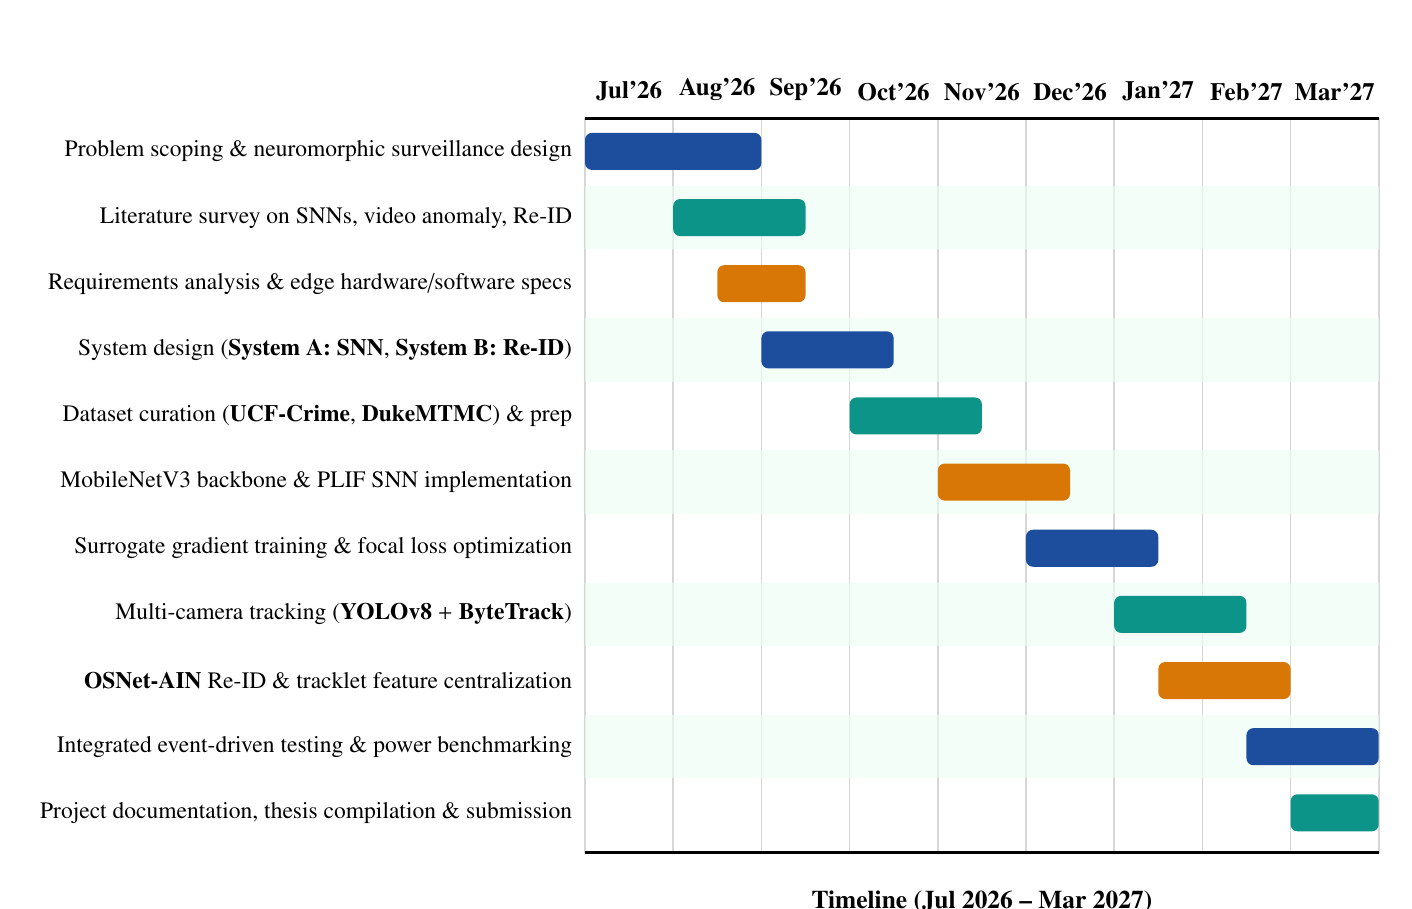
\begin{tikzpicture}[
  x=1.12cm, y=0.84cm,
  lab/.style={anchor=east, font=\fontsize{8.5}{10.5}\selectfont, inner sep=4.5pt, text=black}
]
\def\nm{9}
\def\topY{11.5}

% Vertical month gridlines
\foreach \i in {0,1,...,\nm} {
  \draw[gray!32, line width=0.55pt] (\i, 0.4) -- (\i, \topY);
}

% Month headers on top
\foreach \i/\m in {0.5/Jul'26, 1.5/Aug'26, 2.5/Sep'26, 3.5/Oct'26, 4.5/Nov'26, 5.5/Dec'26, 6.5/Jan'27, 7.5/Feb'27, 8.5/Mar'27} {
  \node[anchor=south, font=\fontsize{9.0}{11.0}\selectfont\bfseries, text=black] at (\i, \topY+0.12) {\m};
}
\draw[black, line width=1.0pt] (0, \topY) -- (\nm, \topY);
\draw[black, line width=0.8pt] (0, 0.4) -- (\nm, 0.4);

% Alternating row background shading
\foreach \k in {0,...,10} {
  \pgfmathsetmacro{\yc}{11.0-\k}
  \ifodd\k
    \fill[prismMint, opacity=0.65] (0, \yc-0.48) rectangle (\nm, \yc+0.48);
  \fi
}

% Task milestone labels on left
\node[lab] at (0, 11.0) {Problem scoping \& neuromorphic surveillance design};
\node[lab] at (0, 10.0) {Literature survey on SNNs, video anomaly, Re-ID};
\node[lab] at (0, 9.0)  {Requirements analysis \& edge hardware/software specs};
\node[lab] at (0, 8.0)  {System design (\textbf{System A: SNN}, \textbf{System B: Re-ID})};
\node[lab] at (0, 7.0)  {Dataset curation (\textbf{UCF-Crime}, \textbf{DukeMTMC}) \& prep};
\node[lab] at (0, 6.0)  {MobileNetV3 backbone \& PLIF SNN implementation};
\node[lab] at (0, 5.0)  {Surrogate gradient training \& focal loss optimization};
\node[lab] at (0, 4.0)  {Multi-camera tracking (\textbf{YOLOv8} + \textbf{ByteTrack})};
\node[lab] at (0, 3.0)  {\textbf{OSNet-AIN} Re-ID \& tracklet feature centralization};
\node[lab] at (0, 2.0)  {Integrated event-driven testing \& power benchmarking};
\node[lab] at (0, 1.0)  {Project documentation, thesis compilation \& submission};

% Milestone Gantt Bars
\fill[prismBlue, rounded corners=2.5pt]     (0.0, 11.0-0.28) rectangle (2.0, 11.0+0.28);
\fill[prismTeal, rounded corners=2.5pt]     (1.0, 10.0-0.28) rectangle (2.5, 10.0+0.28);
\fill[prismGold, rounded corners=2.5pt]     (1.5, 9.0-0.28)  rectangle (2.5, 9.0+0.28);
\fill[prismBlue, rounded corners=2.5pt]     (2.0, 8.0-0.28)  rectangle (3.5, 8.0+0.28);
\fill[prismTeal, rounded corners=2.5pt]     (3.0, 7.0-0.28)  rectangle (4.5, 7.0+0.28);
\fill[prismGold, rounded corners=2.5pt]     (4.0, 6.0-0.28)  rectangle (5.5, 6.0+0.28);
\fill[prismBlue, rounded corners=2.5pt]     (5.0, 5.0-0.28)  rectangle (6.5, 5.0+0.28);
\fill[prismTeal, rounded corners=2.5pt]     (6.0, 4.0-0.28)  rectangle (7.5, 4.0+0.28);
\fill[prismGold, rounded corners=2.5pt]     (6.5, 3.0-0.28)  rectangle (8.0, 3.0+0.28);
\fill[prismBlue, rounded corners=2.5pt]     (7.5, 2.0-0.28)  rectangle (9.0, 2.0+0.28);
\fill[prismTeal, rounded corners=2.5pt]     (8.0, 1.0-0.28)  rectangle (9.0, 1.0+0.28);

% Bottom title
\node[font=\fontsize{9.2}{11.2}\selectfont\bfseries, text=black] at (4.5, -0.35) {Timeline (Jul 2026 -- Mar 2027)};
\end{tikzpicture}
\end{document}
}
    \caption{Project execution schedule and Gantt chart tracking 11 key milestones from July 2026 to March 2027.}
    \label{fig:project_gantt}
\end{figure}

The eleven coordinated work packages executed across the academic timeline were:
\begin{enumerate}
    \item \textbf{Legal Domain Scoping \& Civic Complaint Analysis (Jul--Aug 2026):} Defined legal information access barriers, civic complaint workflows, and user requirements.
    \item \textbf{Literature Survey on RAG Systems, Vector Databases, Legal AI (Aug--Sep 2026):} Reviewed RAG architectures, sentence transformers, vector databases, and multilingual NLP.
    \item \textbf{Requirement Analysis \& Technical Feasibility (Aug--Sep 2026):} Compiled functional and non-functional specifications and technology stack evaluation.
    \item \textbf{System Design (RAG Pipeline, Pinecone, Gemini, FastAPI) (Sep--Oct 2026):} Architected the multi-pipeline system, component dataflows, and schemas.
    \item \textbf{Legal Corpus Acquisition \& PDF Preprocessing (Oct--Nov 2026):} Acquired BNS, BNSS, BSA, RTI, Consumer, Contract, Constitution PDFs and preprocessed text.
    \item \textbf{Embedding Pipeline \& Pinecone Ingestion (all-MiniLM-L6-v2) (Nov--Dec 2026):} Implemented chunking, embedding, normalization, and batch vector upload.
    \item \textbf{Query Processing \& Bilingual Malayalam Translation (Dec 2026--Jan 2027):} Engineered Unicode detection and Gemini-based Malayalam $\leftrightarrow$ English translation.
    \item \textbf{FastAPI Backend Endpoints \& Async Architecture (Jan--Feb 2027):} Developed asynchronous REST endpoints (/, /api/health, /ask, /analyze-document).
    \item \textbf{React 19 + Vite 8 Frontend with Voice Input \& PDF Upload (Jan--Feb 2027):} Created chat interface, Web Speech API integration, and file upload components.
    \item \textbf{Retrieval Evaluation \& Answer Quality Benchmarking (Feb--Mar 2027):} Evaluated retrieval precision, answer accuracy, and citation quality across legal domains.
    \item \textbf{Project Documentation, Report Compilation \& Submission (Feb--Mar 2027):} Compiled comprehensive project report and thesis documentation.
\end{enumerate}


%==============================================================================
% CHAPTER 9: CONCLUSION AND FUTURE SCOPE
%==============================================================================
\chapter{Conclusion and Future Scope}

\section{Conclusion}
This project successfully designed, implemented, and evaluated \textbf{CiviQ}, an AI-powered legal information retrieval system using Retrieval-Augmented Generation. Addressing the challenges of complex statutory language, fragmented document repositories, linguistic barriers, and lack of contextual answers, the platform establishes an accessible legal assistance tool for citizens, students, journalists, and civic organizations.

The core RAG engine leverages \textbf{sentence-transformers (all-MiniLM-L6-v2)} producing 384-dimensional embeddings optimized for semantic search, indexed in \textbf{Pinecone} vector database with HNSW for sub-100ms retrieval. To ensure answer accuracy and prevent hallucination, the system conditions \textbf{Google Gemini 2.5 Flash} generation on retrieved statutory passages, producing grounded responses with explicit citations (Act name, section, clause).

Key accomplishments include:
\begin{itemize}
    \item Overlapping word-chunking (900 words, 150 overlap) preserving legal context across chunk boundaries.
    \item Automatic Malayalam query detection (Unicode U+0D00–U+0D7F) with bidirectional translation, enabling linguistic inclusivity for non-English speakers.
    \item FastAPI asynchronous backend with sub-200ms query latency for question answering and document analysis endpoints.
    \item React 19 + Vite 8 frontend with browser-based voice input (Web Speech API), PDF upload, language selection, top-k slider, and source citation display.
    \item Comprehensive legal corpus including BNS 2023, BNSS 2023, BSA 2023, Consumer Protection Act 2019, Indian Contract Act 1872, RTI Act 2005, and Constitution of India.
\end{itemize}

The system provides citizens with preliminary legal research capabilities previously accessible only through professional legal consultation, democratizing access to statutory knowledge.

\section{Limitations Encountered}
Despite the strong functional capabilities, several technical constraints were encountered:
\begin{itemize}
    \item \textbf{Retrieval Quality Dependence:} Answer accuracy is bounded by retrieval precision. Queries requiring cross-statute synthesis (e.g., connecting Contract Act obligations with Consumer Protection remedies) may miss relevant passages if chunk embeddings are insufficiently similar.
    \item \textbf{Malayalam Translation Nuance:} Legal terminology translation (e.g., ``consideration,'' ``specific performance'') sometimes loses technical precision in Malayalam, requiring manual review for domain-critical terms.
    \item \textbf{Image-Only PDF Limitation:} Scanned legal documents without embedded text (image-only PDFs) cannot be processed without OCR preprocessing, excluding older archival statutes.
    \item \textbf{No Case Law Integration:} The current corpus focuses on statutes; judicial precedents and Supreme Court judgments are excluded, limiting applicability for nuanced legal interpretation.
\end{itemize}

\section{Future Scope}
Future enhancements to expand and advance the platform include:
\begin{itemize}
    \item \textbf{Fine-Tuning Legal Domain Embeddings:} Training a legal-domain-specific sentence transformer on Indian statutory corpora to improve embedding quality for legal terminology and cross-references.
    \item \textbf{Expanding Regional Language Support:} Adding Tamil, Telugu, Hindi, Kannada, and Bengali translation pipelines to serve diverse Indian linguistic communities.
    \item \textbf{Incorporating Judicial Precedents:} Integrating Supreme Court and High Court judgment databases to provide case law citations alongside statutory references.
    \item \textbf{Building User Feedback Loops:} Implementing thumbs-up/down rating for answer quality and retrieval relevance to continuously improve the system through reinforcement learning from human feedback (RLHF).
    \item \textbf{RTI Portal Integration:} Connecting with government RTI portals to enable automated filing of information requests with pre-filled forms based on user queries.
    \item \textbf{Deploying Mobile Applications:} Developing native Android and iOS applications with offline fallback for basic legal reference in areas with limited internet connectivity.
\end{itemize}


%==============================================================================
% REFERENCES
%==============================================================================
\begin{thebibliography}{99}
\sloppy

\bibitem{ref_rahman2025_legalqueryrag}
R. S. M. Wahidur, S. Kim, H. Choi, D. S. Bhatti, and H.-N. Lee, "Legal Query RAG," \textit{IEEE Access}, vol.~13, pp.~3542125, February 2025.

\bibitem{ref_mubeen2025_legalease}
F. Mubeen, A. Mehdi, M. A. Haque, M. Z. M. Nomani, and N. S. Uddin, "Redefining legal access: A RAG-based AI system for Indian law," \textit{Human-Intelligent Systems Integration}, vol.~7, no.~2, pp.~87--98, October 2025.

\bibitem{ref_nigam2026_ailqa}
S. K. Nigam, S. K. Mishra, N. Shallum, K. Ghosh, and A. Bhattacharya, "AILQA: Evaluating AI-driven legal question answering systems for the Indian legal system," \textit{Artificial Intelligence and Law}, vol.~34, pp.~1--28, July 2026.

\bibitem{ref_bhattacharya2025_ardi}
U. Bhattacharya, A. Deroy, A. Bandyopadhyay, G. Majumdar, S. K. Guha, K. Rudra, S. Ghosh, and K. Ghosh, "ARDI: A new dataset for automatic advocate recommendation in the Indian legal system," \textit{Artificial Intelligence and Law}, vol.~33, pp.~1--29, August 2025.

\bibitem{ref_ren2026_autodata}
W. Ren, L. Shen, J. Zhu, S. Li, Y. Hong, J. Wang, and D. Cao, "Automated data synthesis and retrieval-augmented generation for legal large language models," \textit{Knowledge-Based Systems}, vol.~347, art.~no.~116267, May 2026.

\bibitem{ref_italiani2025_enhancing}
P. Italiani, G. Moro, and L. Ragazzi, "Enhancing legal question answering with data generation and knowledge distillation from large language models," \textit{Artificial Intelligence and Law}, vol.~33, no.~4, pp.~1--24, April 2025.

\bibitem{ref_webb2026_genai}
J. Webb, "Generative artificial intelligence in legal practice: Epistemic expertise, unethical AI, and the role of virtue," \textit{Minds and Machines}, vol.~36, no.~1, art.~no.~19, March 2026.

\bibitem{ref_linders2025_kg_rag}
J. Linders and J. M. Tomczak, "Knowledge graph-extended retrieval augmented generation for question answering," \textit{Applied Intelligence}, vol.~55, no.~12, art.~no.~1102, November 2025.

\bibitem{ref_thambi2024_lawgic}
A. S. Thambi, A. Devangavi, R. Pankaja, and A. Joshi, "‘LAWGIC’: An application for automated legal document classification and retrieval," \textit{Journal of Electronics and Informatics}, vol.~6, no.~2, pp.~157--170, June 2024.

\bibitem{ref_gupta2024_legalassist}
J. Gupta, A. Sharma, S. Singhania, and A. I. Abidi, "Legal Assist AI---Leveraging transformer based model for effective legal assistance," \textit{Research Square Preprint}, DOI: 10.21203/rs.3.rs-5351879/v1, November 2024.

\bibitem{ref_song2025_summarization}
Y. Song, Y. Qin, R. Huang, Y. Chen, and C. Lin, "Legal text summarization via judicial syllogism with large language models," \textit{Journal of King Saud University---Computer and Information Sciences}, vol.~37, no.~7, art.~no.~111, July 2025.

\bibitem{ref_garg2026_multifaceted}
S. Garg, H. Bysani, S. S. Chandana, Y. G. Prasoona, D. Gupta, S. Vekkot, and S. Sinha, "Multifaceted structural classification of Indian legal judgments," \textit{Discover Artificial Intelligence}, vol.~6, no.~1, art.~no.~282, February 2026.

\bibitem{ref_sha2026_rhetorical}
S. A. A. Sha, S. Sivanesan, A. K. Madasamy, and N. Binu, "Rhetorical-role-aware retrieval-augmented generation for legal question answering over Indian Supreme Court judgments," \textit{arXiv preprint arXiv:2608.06828}, August 2026.

\bibitem{ref_dhanani2022_scalable}
J. Dhanani, R. Mehta, and D. Rana, "Effective and scalable legal judgment recommendation using pre-learned word embedding," \textit{Complex \& Intelligent Systems}, vol.~8, no.~4, pp.~3199--3213, February 2022.

\bibitem{ref_singh2026_transformer_xai}
R. A. Singh and J. N. Dwivedi, "A novel transformer-XAI framework with bias attribution and A-RAG for Indian judicial system," \textit{Discover Applied Sciences}, vol.~8, no.~7, art.~no.~9150, June 2026.

\end{thebibliography}

\end{document}
